\documentclass[12pt,twoside]{report}

% some definitions for the title page
\newcommand{\reporttitle}{The Emotion Engine}
\newcommand{\reportauthor}{Kaede Sugano}
\newcommand{\supervisor}{William Knottenbelt}
\newcommand{\reporttype}{Undergraduate Individual Project}
\newcommand{\degreetype}{MEng} 

% load some definitions and default packages
\input{includes}

% load some macros
\input{notation}

% load title page
\begin{document}
\input{titlepage}


% page numbering etc.
\pagenumbering{roman}
\clearpage{\pagestyle{empty}\cleardoublepage}
\setcounter{page}{1}
\pagestyle{fancy}

%%%%%%%%%%%%%%%%%%%%%%%%%%%%%%%%%%%%
\begin{abstract}
Language inevitably compresses and simplifies human emotion, causing subtle affective nuances to be lost in verbal expression. Although large language models (LLMs) can recognise and generate emotional language, most existing methods rely on discrete emotion labels or token-level control, which limits fine-grained and intuitive affective manipulation.

This project proposes an Emotion Engine that represents emotion as a continuous latent vector, rather than explicit linguistic categories. Given an input text, the system extracts its underlying emotional state as a low-dimensional emotion vector, which composes multiple overlapping affective directions. Users can directly adjust intensities of those vectors before regenerating text, that reflects the edited emotional state. Importantly, this operation is performed prior to language generation, bypassing the lossy compression inherent in verbalisation.

By leveraging recent advances in latent-space reasoning and internal activation steering in LLMs, the Emotion Engine enables controllable, pre-verbal emotion editing within a text-to-text pipeline. Human communication is always mediated by media. This project can affect all communication in the sense that it deals with feelings evoked by the media. Recent creative act with LLM prompt engineering may in fact be a role reversal, since creativity should serve before the verbalisation. By making it possible to edit the feelings that were really wanted to be conveyed, this project could bring about a more precise communication that society has never seen before.

\end{abstract}

\cleardoublepage
%%%%%%%%%%%%%%%%%%%%%%%%%%%%%%%%%%%%
\section*{Acknowledgments}
Comment this out if not needed.

\clearpage{\pagestyle{empty}\cleardoublepage}

%%%%%%%%%%%%%%%%%%%%%%%%%%%%%%%%%%%%
%--- table of contents
\fancyhead[RE,LO]{\sffamily {Table of Contents}}
\tableofcontents 


\clearpage{\pagestyle{empty}\cleardoublepage}
\pagenumbering{arabic}
\setcounter{page}{1}
\fancyhead[LE,RO]{\slshape \rightmark}
\fancyhead[LO,RE]{\slshape \leftmark}

%%%%%%%%%%%%%%%%%%%%%%%%%%%%%%%%%%%%
\chapter{Introduction}
\section{Words draw boundary lines across the ocean of ``concepts''}
When I was still in elementary school, my favourite biography in the library was Helen Keller’s. Stricken by illness as a child, she lost both sight and hearing and bore the ``triple hardship'' of being blind, deaf, and mute, yet devoted herself to the advancement of education and welfare for the disadvantaged.

But Helen Keller’s story is not merely a tale of ``overcoming adversity.'' What is etched most vividly in my memory is the moment when she first understood the word ``water.'' At first, Helen insisted that ``cup'' and ``the water in it'' were the same thing. However, the instant when Anne Sullivan signed ``W-A-T-E-R'' into her hand while letting the cold water from a pump run across Helen’s palm, her world changed. When she could separate the object that flows from the container, the continuum of chaos was reshaped into an ordered world with partitions.

This scene exemplifies the essence of language. We do not grasp the external world directly as ``things-in-themselves.'' The information flowing into our senses is, in truth, a continuum; language draws borders there and carves out units of meaning. Even the boundary between river and sea is not sharply inscribed by nature itself; it is defined for human convenience and by culture~-- ``this far is river,'' ``from here is sea.'' Words do not merely copy lines already inscribed upon the world; they are the very act of drawing those lines as needed. In other words, language is not just a label: it is the activity by which we impose boundaries within our cognition and shape the world we see. To learn words is not merely to expand vocabulary; it is to gain a way of partitioning the ocean of concepts and choosing how to look at the world. In that sense, we are, day by day, sketching new boundaries.

\section{Verbalisation is a lossy compression}
Verbalisation is an act of forcing the complex and continuous sensation into discretised vocabulary and grammar. When we perform \textbf{verbalisation}, there lurks a commonly overlooked risk; it is intrinsically \textbf{lossy}. The moment we verbalise, the fine nuances contained within raw feeling are abstracted into the fences of cognition that humanity has drawn at the level of words. Even if we choose the same term, the warmth that term carries depends on each person’s embodied history, and it is eventually averaged out. The relief or pride we felt when we opened our old school yearbook for the first time in a decade, once put into text, may be flattened into a bland ``how nostalgic.'' Moreover, lexicons and meanings for emotions differ greatly across languages and cultures\cite{jackson2019emotion}; terms like ``anger'' or ``joy'' do not necessarily point to the same nuances around the world. And yet humanity cannot let go of language. Even if it is a lossy compression, language remains the only standardised interface that connects the human heart to society.


\section{Objectives}
The goal of this project is not to deny language but to design a parallel circuit that supplements the components lost in the compression of verbalisation, i.e.\ a circuit for restoring what words leave behind. What if we could scoop up the human central cognition directly, without passing through the rendering pipeline of language, and translate it into other forms of expression? Could we transfer the lingering sensation that arises when reading a letter from your significant other into poetry or essays? Or could we improve novel translations by capturing emotions lost through differences in lexical definitions between languages? Here lies an uncharted gap in our understanding of human cognition. 

This project aims to emulate a kind of human synaesthesia. In other words, we aim to map emotions across modalities. We will develop the foundational technology to extract, manipulate, and re-synthesise a \textbf{pre-verbal, intermediate representation of emotion}, and explore possible ways to steer the model output using those representations of emotion.

The final product of this project is a computational system capable of extracting, manipulating, and presenting the emotions contained in input text without having to go through the compression of verbalisation.
The system focuses not on what the text superficially tells, but on the emotional state that existed immediately before the text was produced, and treats it as a continuous vector representation.

When a user enters any text, the system analyses the emotional nuances contained in that text and visualises them as a low-dimensional continuous vector. These emotion vectors are not discrete labels such as ``joy'' and ``sadness,'' but are expressed as multiple overlapping emotional directions, thus preserving subtle mixed emotions and fluctuations that cannot be captured by language.

Users can intuitively manipulate this emotion code space. For example, by strengthening only a specific emotional direction and weakening another direction for the simultaneous presence of \texttt{relief} and \texttt{loneliness} in a certain sentence, it is possible to sensitively edit the emotional state that one really wanted to convey. It is important to note that this operation is not performed at the linguistic level, such as vocabulary selection or stylistic adjustment, but rather on the emotional expression itself before the language is generated.

The edited emotion code is again transformed into a linguistic expression. The text generated here is not simply a paraphrased sentence, but is the result of a re-expression that retains or intentionally transforms the emotion contained in the original sentence.

In this process, the user does not need to put their emotions into explicit words. The verbal averaging and simplification that is usually considered inevitable between emotion recognition and generation is bypassed, and the raw emotion felt by the user can be transferred to another form of expression in a more controllable manner.

This end product is neither a system for classifying and diagnosing emotions nor a tool for automatically generating emotional sentences. Rather, it is an interface that temporarily holds the emotions that people had before they put them into words as manipulatable intermediate expressions, from which new linguistic expressions can be launched. The ultimate value of this project lies in the fact that it makes it possible to return to the boundaries drawn by language and choose words again.


%%%%%%%%%%%%%%%%%%%%%%%%%%%%%%%%%%%%
\chapter{Background}

\section{Emotion Representation in LLMs}

\subsection{Discrete Emotion Labels and Their Limitations}

Early work treated emotion as a small set of discrete categories. The most influential taxonomy is Ekman’s seven basic emotions: anger, contempt, disgust, enjoyment, fear, sadness, and surprise~\cite{ekman1999basic}. 

\begin{figure}[H]
    \centering
    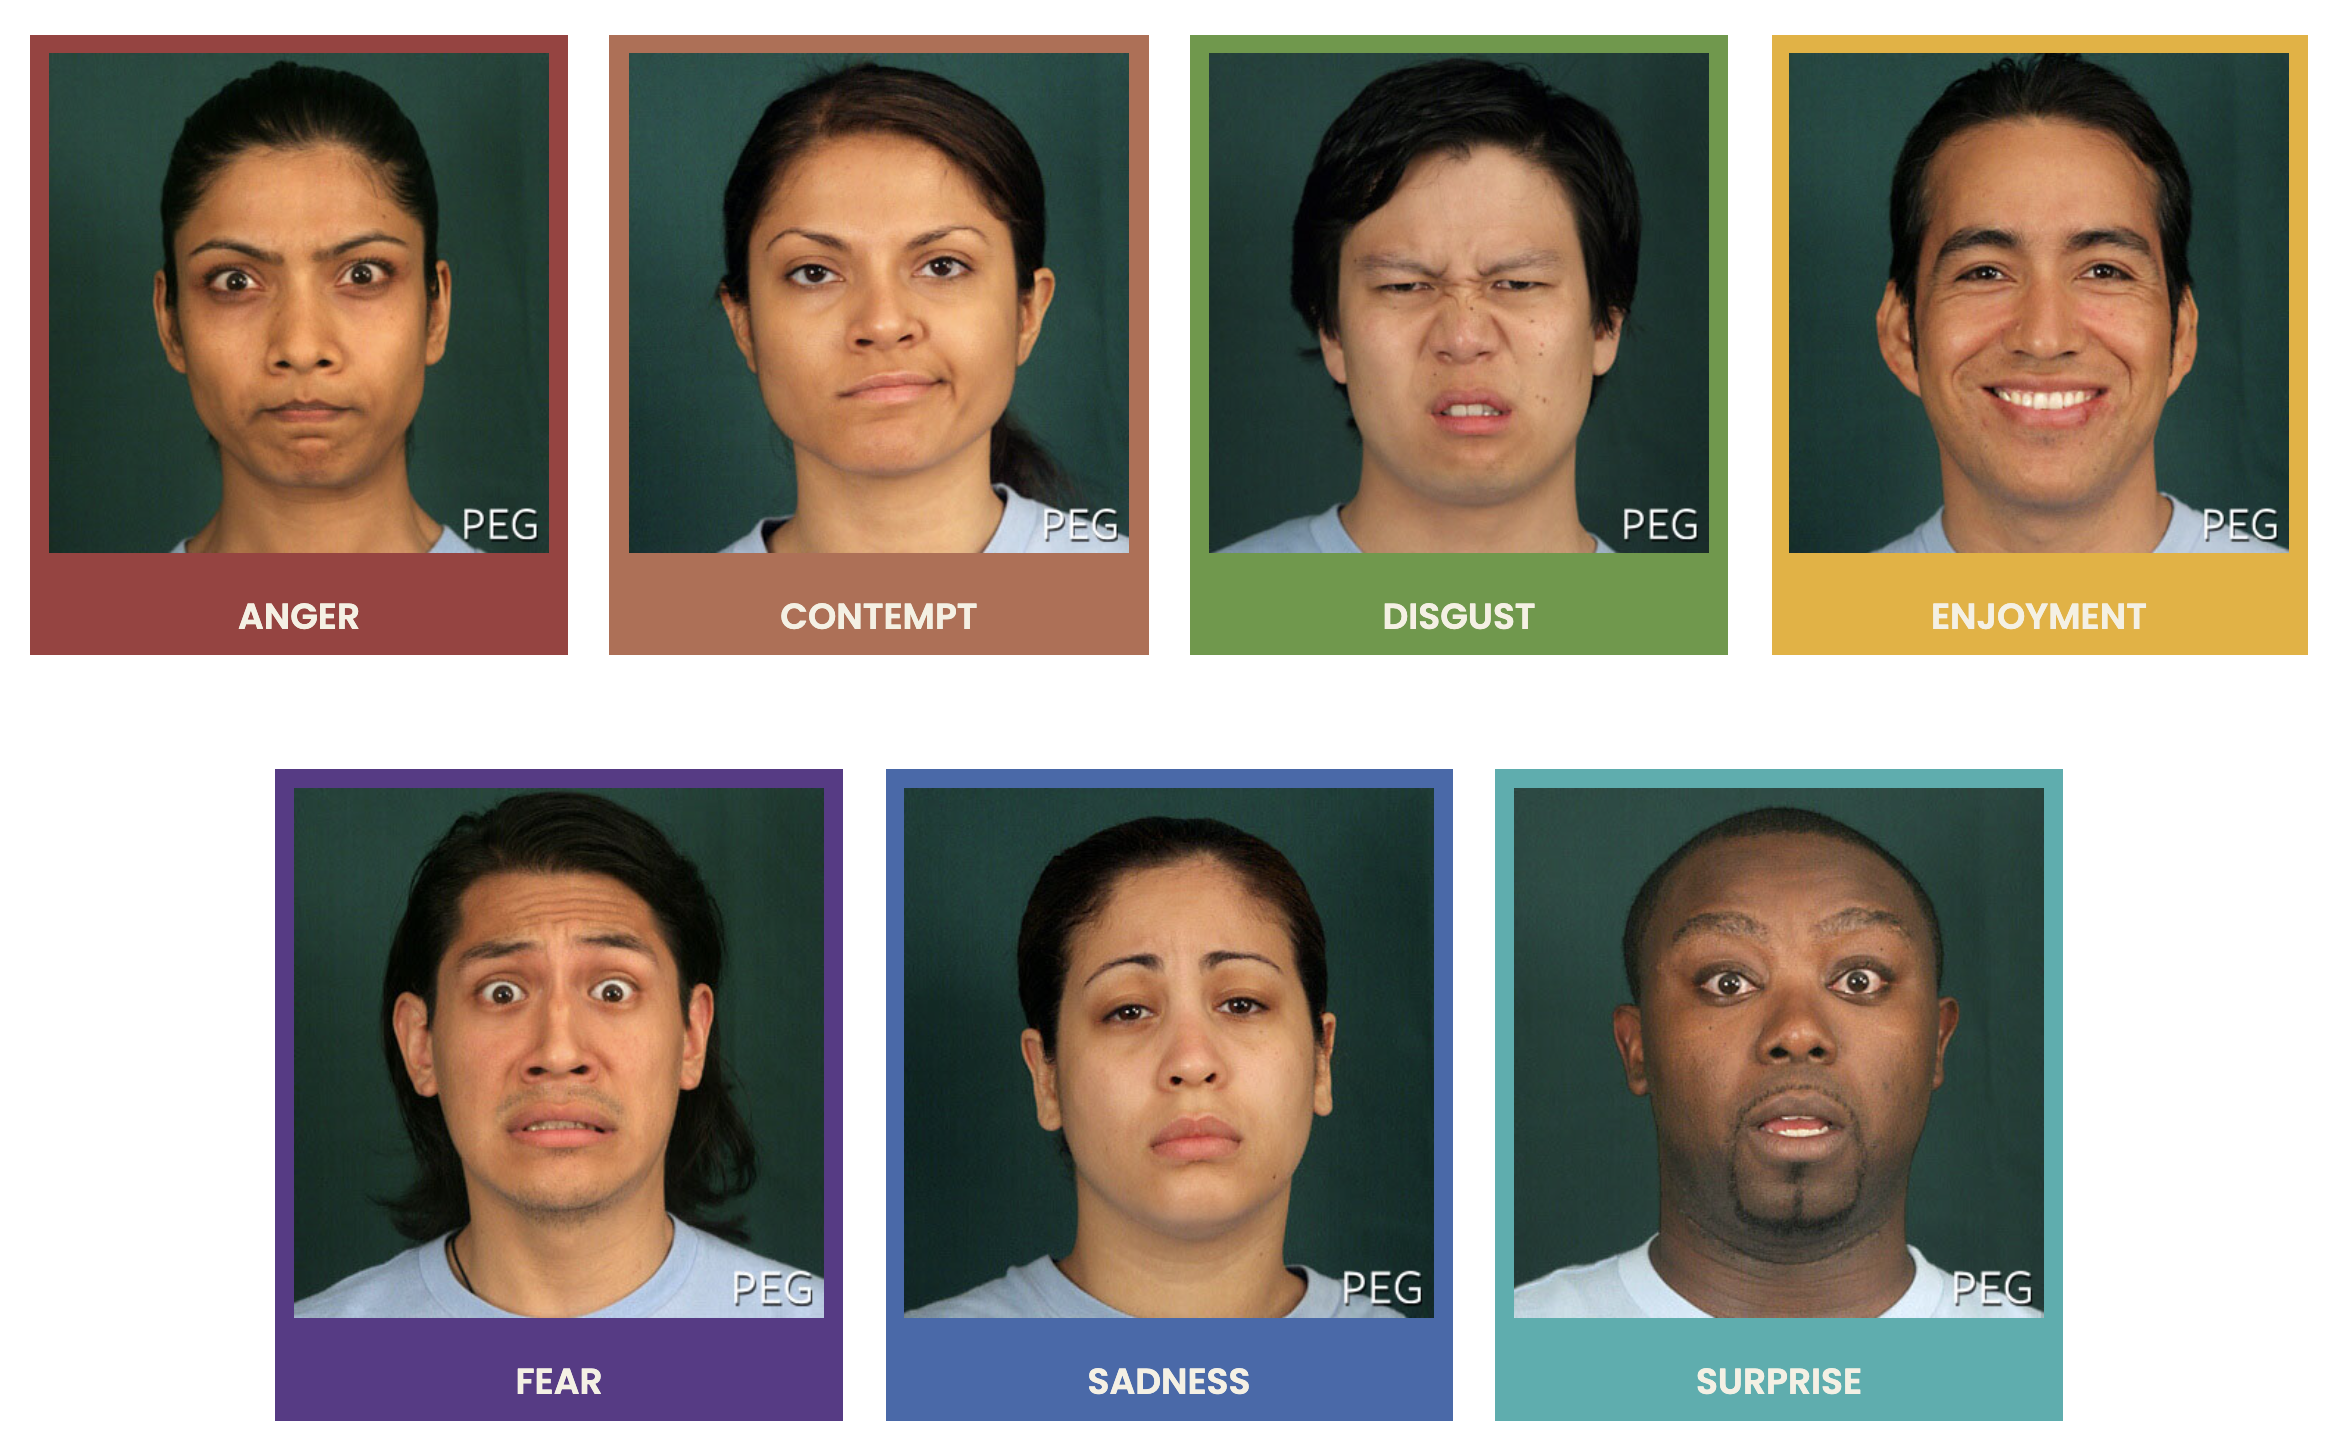
\includegraphics[width=0.5\linewidth]{figures/paul_ekman.png}
    \caption{Paul Ekman's seven basix emotions~\cite{paul_ekman_web}}
    \label{fig:paul_ekman}
\end{figure}

This assumes that emotions are biologically universal and psychologically irreducible. This framework enabled early supervised emotion classification systems by providing a clear labeling scheme and facilitated the construction of benchmark datasets. However, the categorical assumption introduces strong inductive bias; emotions are treated as mutually exclusive and qualitatively distinct.

Subsequent datasets attempted to increase expressive granularity. GoEmotions~\cite{demszky2020goemotionsdatasetfinegrainedemotions}, for example, expanded the label space to 27 emotion categories and allowed multi-label annotation. 

\begin{figure}[H]
    \centering
    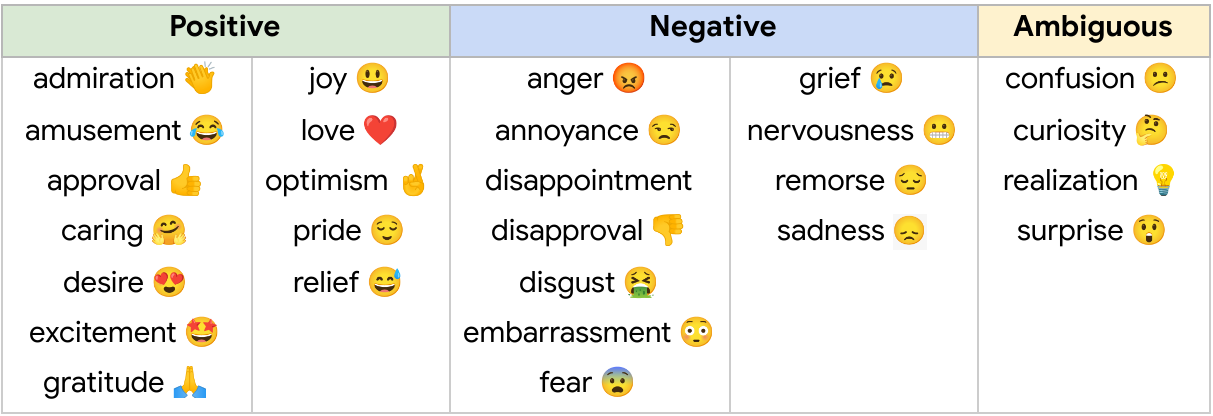
\includegraphics[width=0.8\linewidth]{figures/goemotions.png}
    \caption{GoEmotions taxonomy: 28 emotion categories including ``neutral''.~\cite{goemo}}
    \label{fig:goemotions}
\end{figure}

This enabled us to capture cases where multiple emotions occur in a single utterance. It is reported that emotions cluster by sentiment polarity and intensity, and that many categories exhibit high inter-label correlation. Nevertheless, despite its increased resolution, the dataset still relies on one-hot / sparse multi-hot encodings. Such encodings collapse emotional intensity and compositional structure into discrete indices, preventing the representation of graded transitions. For example, the difference between mild and intense anger cannot be represented, and the blend of emotions, such as bittersweet emotion, is also difficult.

Essentially, discrete labels force the learning problem into a classification regime that cannot capture continuity, geometry, or arithmetic structure. For example, two samples labeled \texttt{joy} may be emotionally distant, while \texttt{joy} and \texttt{contentment} may be emotionally close; yet this structure is invisible to the model itself. These limitations motivate a shift away from purely categorical representations toward continuous emotion spaces.

This problem of the discretised emotion labels is also raised  by Wang and Zong (2021)~\cite{wang-zong-2021-distributed}. They explicitly formalise this by arguing that one-hot emotion labels ignore latent relationships between emotion categories. They observe that emotion calsses are not orthogonal in human perception, but rather exhibit similarity in a gradation manner. More broadly, discrete labeling schemes prioritises  the annotation convenience over the representational adequacy. While it simplify supervision and evaluation, they impose artificial bounadies that obscure the underlying structure of emotions. This mismatch becomes especially problematic when attempting cross-dataset transfer or cross-cultural comparison, where differences in label granularity cannot be reconciled within a purely categorical framework.

These shortcomings have motivated a growing body of work that seeks to represent emotion in continuous spaces, where distance, direction, and magnitude encode affective relationships. By having a representation methods that preserves intensity, similarity and compositionality, we can enable models to capture nuanced emotional variation beyond rigid class boundaries. This transition from discrete labels to continuous emotion spaces is the focus of the next subsection.

\subsection{From Discrete Labels to Continuous Emotion Spaces}

Continuous emotion representations seek to encode emotion as points in a low-dimensional vector space, where distance, direction, and magnitude correspond to psychological relationships. Early psychological models such as the pleasure–arousal–dominance (PAD) framework~\cite{MehrabianRussell1974} formalised emotion along continuous axes, suggesting that emotions differ quantitatively rather than categorically.

\begin{enumerate}
    \item \textbf{Pleasure} represents the hedonic quality of an experience, ranging from unpleasant to pleasant. States such as joy, contentment, and satisfaction occupy the positive end of the pleasure axis, whereas sadness, disgust, and despair lie toward the negative end.
    \item \textbf{Arousal} captures the degree of physiological and cognitive activation associated with an emotional state, ranging from calm or lethargic to excited or agitated. High-arousal states include fear, anger, and excitement, while low-arousal states include relaxation, boredom, or melancholy. 
    \item \textbf{Dominance} reflects the extent to which an individual feels in control of, or overpowered by, a situation. High-dominance states are associated with feelings of agency, confidence, and control (e.g. pride, anger), whereas low-dominance states correspond to submission, helplessness, or vulnerability (e.g. fear, shame). 
\end{enumerate}

Together, these three dimensions define a continuous affective space in which canonical emotion categories correspond to regions rather than points. For example, anger and fear are both negatively valenced and highly aroused, but are separable along the dominance axis; sadness and boredom share low arousal and negative valence, but differ in dominance and intensity. This geometric interpretation naturally accounts for graded emotional intensity, mixed emotions, and smooth transitions between affective states~-- phenomena that are difficult to represent with discrete labels.

\begin{figure}[H]
    \centering
    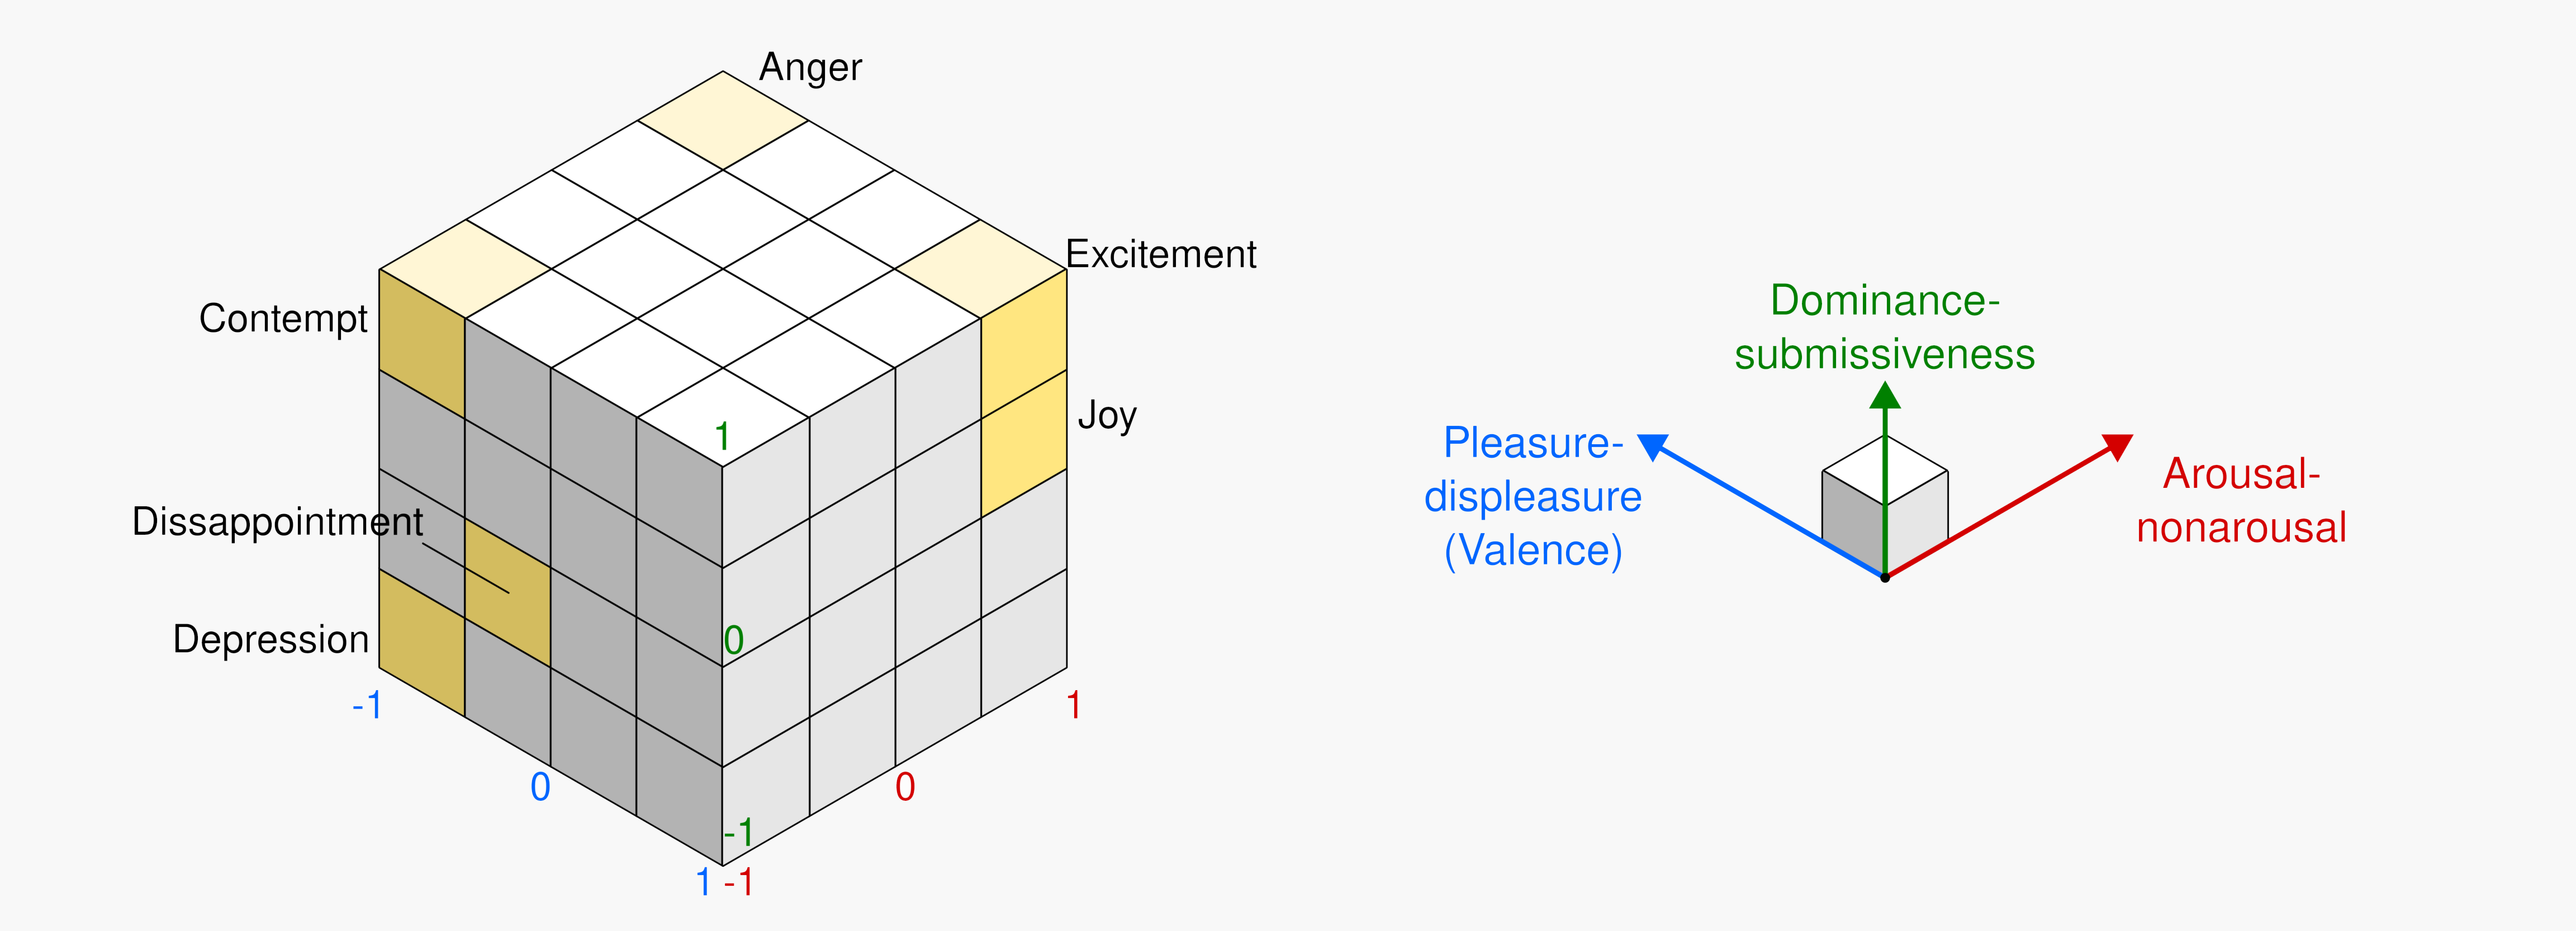
\includegraphics[width=0.8\linewidth]{figures/pad.png}
    \caption{Representation of PAD model done with cubes~\cite{pad}}
    \label{fig:pad}
\end{figure}

Additionally, in the field of affective computing, an explicit attempt to bridge the gap between discrete labels and continuous emotion representations is presented by Buechel et al.~\cite{buechel2021labelagnosticemotionembeddings}. Rather than committing to a single emotion taxonomy, they propose learning \emph{label-agnostic emotion embeddings} that serve as a shared latent representation across heterogeneous annotation schemes, including polarity, basic emotion categories, and affective dimensions such as valence and arousal.

Crucially, emotion labels in this framework are not treated as targets to be predicted directly, but as projections from a common embedding space. Models are trained to map text into this latent affective space, from which multiple label formats can be recovered via lightweight prediction heads. This design enables the learned emotion information to be transferred to another without retraining the full model. Empirically, Buechel et al.\ show that such embeddings preserve prediction quality while supporting cross-dataset generalisation.

Complementary to this, Wang and Zong (2021)~\cite{wang-zong-2021-distributed} focus on learning continuous representations for \emph{emotion categories themselves}. Instead of representing emotion classes as one-hot vectors, they derive distributed emotion embeddings by averaging soft classifier outputs over all instances of a given emotion category. These representations form an emotion space in which distances reflect empirical similarity between emotions as expressed in text. Their results demonstrate that emotion categories cluster by sentiment polarity and intensity, which captures the emotions more faithfully than the conventional semantic word embedding spaces. 

Both of those approaches we looked at enable emotion to be represented as a continuous, low-dimensional structure where each of them corresponds to a region or a direction in a metric space. This perspective aligns closely with psychological theories such as PAD, while remaining grounded in data-driven learning from natural language.

Importantly, representing emotion in continuous spaces shifts the learning problem away from rigid classification toward geometric representation learning. This not only resolves many of the limitations inherent in discrete labels, but also provides a foundation for analysing how emotional information is encoded in vector representations more generally. In particular, it raises the question of whether emotion occupies identifiable subspaces or linear directions within learned embeddings, a topic explored in the following subsection.

\subsection{Linear Structure of Emotion in Word Embedding Spaces} \label{linear_word_embedding}

An important question here is whether the continuous space for emotion is actually reflected in learned language representations. Interestingly, prior to the emergence of LLMs, static word embeddings already exhibited evidence of latent affective organisation, despite being trained without explicit emotional supervision.

Wu and Jiang~\cite{linear_vector_emo} demonstrate that emotional information in word embeddings such as GloVe~\cite{brochier2019global} is not uniformly distributed across dimensions, but instead concentrated along a small number of linear directions. They train a linear autoregressive model to predict continuous emotional valence on annotated narrative data, and show that only a limited subset of embedding dimensions contributes to emotional valence. Interpreting the learned weights reveals that emotional polarity can be captured by a low-dimensional subspace embedded within the full semantic space.

It is also reported that projecting word embeddings into this learned emotion subspace produces a substantially clearer separation between positive and nefative emotion. This indicates that emotion is linearly recoverable even when embeddings are trained without affective objectives. Namely that, emotional meaning is encoded \textbf{geometrically}, rather than a byproduct of lexical associations.

A particularly significant finding is that this projected emotion space preserves \emph{linear compositional structure}. Vector arithmetic over words that contain emotion yields composite affective states, which is also consistent with psychological theories of emotion composition such as Plutchik’s wheel of emotions~\cite{plutchik1980emotion}.

\begin{figure}[H]
    \centering
    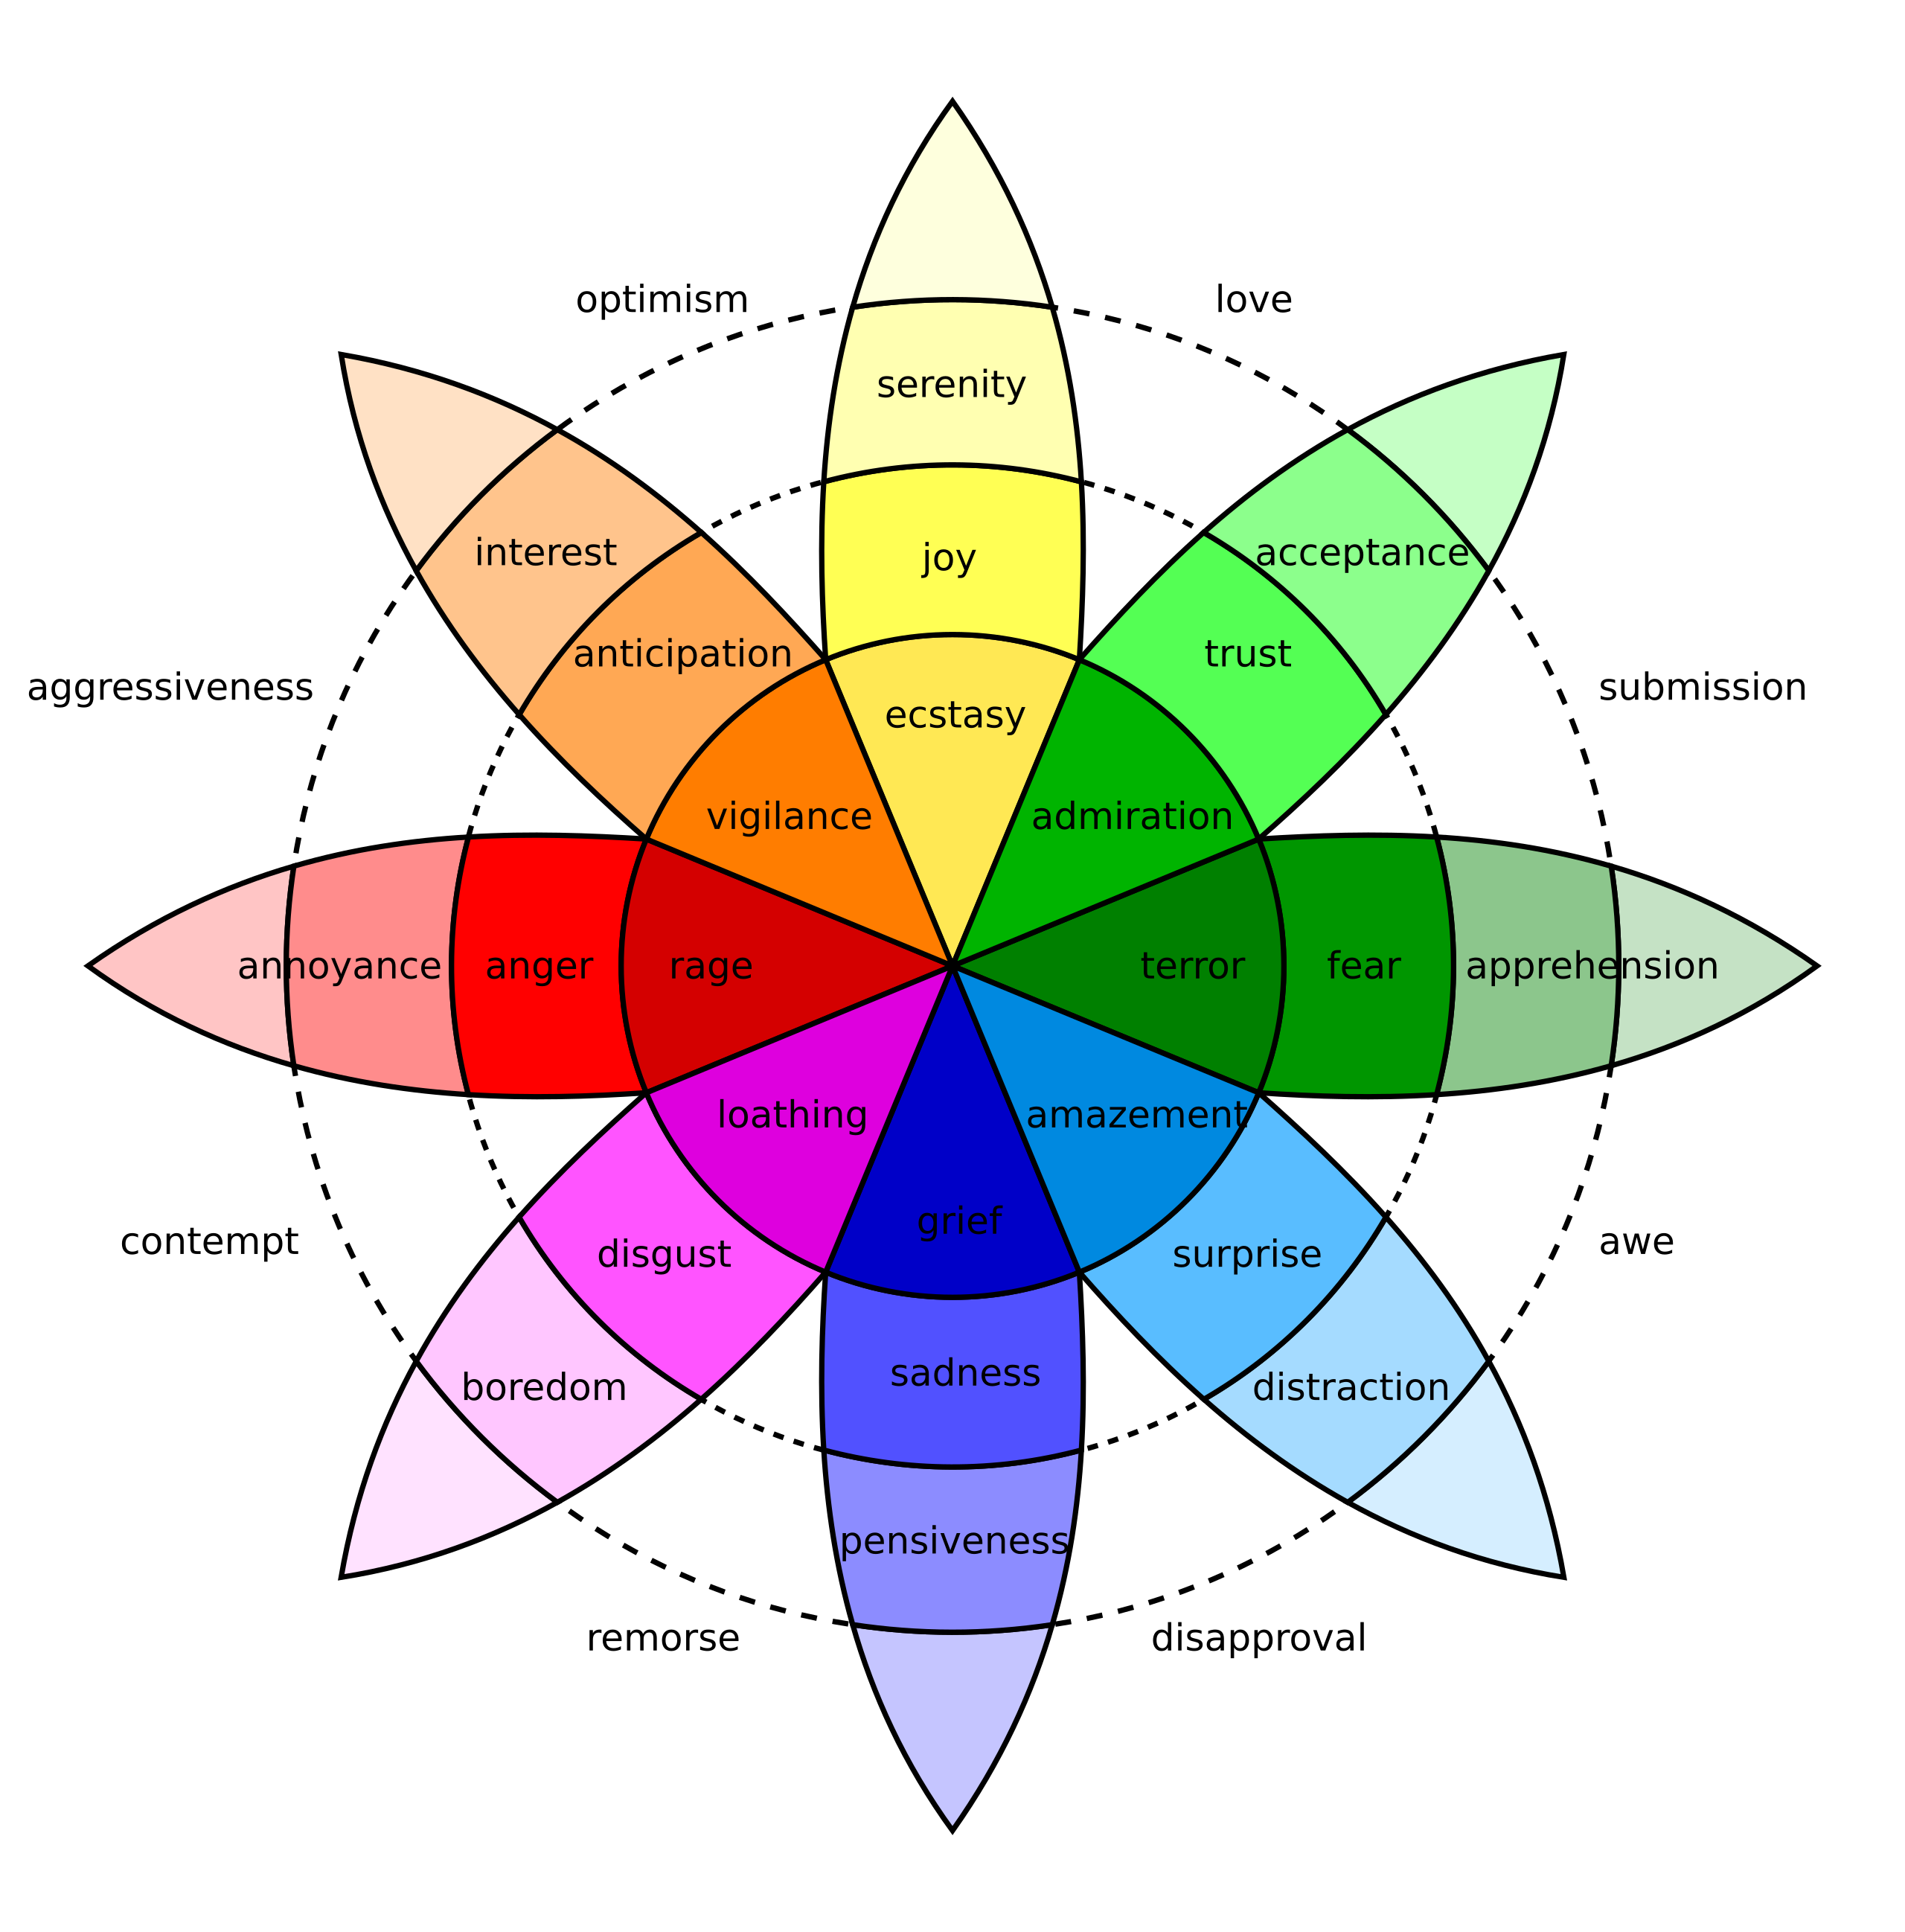
\includegraphics[width=0.5\linewidth]{figures/Plutchik-wheel.png}
    \caption{Plutchik’s wheel of emotions: basic emotions are arranged radially, with angular proximity indicating similarity and radial intensity indicating emotional strength.}
    \label{fig:Plutchik}
\end{figure}

For example, the vector sum of \texttt{joy} and \texttt{trust} aligns closely with \texttt{love}, while remaining distant from affectively opposing states such as \texttt{remorse}. This behaviour cannot be captured by categorical representations, but emerges naturally in a continuous, vector-valued framework.

These results indicate that emotion in word embedding spaces is not only continuous but also approximately linear, admitting meaningful projections, directions, and arithmetic operations. As a result, affective similarity, intensity, and composition can be expressed through simple linear operations rather than discrete class boundaries.

Taken together, these findings provide early evidence that emotion is encoded as structured geometry within learned language representations. This establishes a representational bridge between psychological models of emotion and mathematical embedding paradigms. This also motivates further research into how such linear emotional structure scales and evolves in more expressive representation learning systems.

\section{Manipulation of Latent Representations}

To harness these emotion vectors, researchers have explored techniques for directly manipulating internal representations of models.

\subsection{Neuron-Level Emotion Control}

One line of work focuses on exploiting localised affective representations at the neuron level. For instance, Radford et al.\ (2017)~\cite{radford2017learninggeneratereviewsdiscovering} noted a single ``sentiment neuron'' in a byte-level recurrent language model. It has shown that the activation strongly correlates with review polarity and the manipulation of that sentiment neuron directly controls the generated sentiment. Later work shows that modern LLMs contain clusters of neurons selectively responsive to specific emotions. 

Ablation and masking experiments were done by Lee et al.\ (2025)~\cite{lee-etal-2025-large}, and it demonstrates that removing these neurons can selectively impair recognition of particular emotions. This confirms that they play a functional role rather than being incidental correlates. However, there is still a possibility that the model is redundant. For some emotions, performance remains stable after ablation, suggesting overlapping representations and compensatory mechanisms.

Additionally, low-resource fine-tuning methods such as LoRA (Low-Rank Adaptation)~\cite{hu2021loralowrankadaptationlarge} and prefix-tuning operate at a higher level of abstraction but still manipulate latent activations. By injecting small learned vectors into the model we can induce a consistent emotional tone without full retraining. This shows that affective style is encoded in directions that are easy to steer with low-rank updates.

\subsection{Emergent Emotional Subspaces in Large Language Models}

Large language models substantially extend and generalise the affective structure previously observed in static word embeddings (\ref{linear_word_embedding}). Even though models are trained on massive corpora without any emotional information supervision, LLMs acquire rich contextual representations. These models appear to internalise emotion as a continuous and distributed property of their hidden-state geometry.

Recent work provides strong empirical evidence for this claim. Reichman et al.\ (2025)~\cite{reichman2025emotionsartthouunderstanding} show that emotional information in large decoder-only LLMs is organised within a low-dimensional \textbf{emotional manifold} embedded in the activation. 

They analysed hidden states across layers, demonstrated how affective content aligns with a small number of stable latent directions. Importantly, these directions appeared without any explicit emotion supervision, indicating that affective structure is a natural consequence of large-scale language modelling rather than a task-specific artefact. Moreover, the identified emotional subspace is remarkably consistent across domains and languages, suggesting that LLMs internalise a broadly universal affective geometry.

Crucially, this geometry is not merely descriptive. Reichman et al.~\cite{reichman2025emotionsartthouunderstanding} show that small interventions along these latent directions can alter the model’s emotional interpretation of an input, while preserving its semantic content. This establishes emotional subspaces as functionally meaningful components of the model’s representation space, rather than passive correlates of surface-level sentiment cues. This establishes emotional subspaces to be considered as a functional and meaningful components of the model’s representation space.

Complementary evidence comes from neuron-level analyses too. Lee et al.\ (2025)~\cite{lee-etal-2025-large} identify groups of neurons whose activations selectively track specific basic emotions in large instruction-tuned models. Emotional information is broadly distributed, but certain neurons constantly exhibit disproportionately strong responses to particular affective states. Further ablation experiments revealed that suppressing these neurons can significantly degrade emotion recognition performance for some emotions. This provides a causal evidence that emotional information is actively processed rather than epiphenomenal.

Taken together, these findings suggest that emotion in LLMs is best characterised as an emergent, low-dimensional subspace embedded within high-dimensional contextual representations. Emotional meaning is not localised to single units, nor reducible to discrete labels; instead, it occupies a structured region of stable latent space. This emergent affective geometry provides the representational foundation that enables direct control of emotional behaviour through linear interventions, which we discuss next.

\subsection{Steering Latent States with Linear and Continuous Control Vectors}

If emotional meaning in LLMs is encoded as directions or subspaces within latent representations, a natural consequence is that affective behaviour should be directly controllable by intervening along those directions. This observation has motivated a line of work on \textbf{latent steering}, in which linear and continuous control vectors are applied directly to internal activations during inference.

An early and influential approach is Plug-and-Play Language Models (PPLM)~\cite{dathathri2020plugplaylanguagemodels}, combines a frozen language model with an external attribute model (e.g.\ a sentiment classifier) and performs gradient ascent on the hidden states to increase the likelihood of a desired attribute. Effectively, this method introduces a small \textbf{sentiment vector} into the latent representation, biasing generation toward positive or negative emotion without modifying the model’s weights. Although originally framed as a controllable generation technique, PPLM implicitly relies on the assumption that affective attributes correspond to approximately linear directions in latent space.

More recent work makes this assumption explicit and removes the need for iterative optimisation. Anthropic’s \textbf{Contrastive Activation Addition} (CAA)~\cite{caa} directly intervenes in a model’s internal activations using precomputed \textbf{steering vectors}. These vectors are obtained by collecting large sets of positive and negative examples of a target behaviour or attribute and averaging the differences in their intermediate representations. The resulting vector captures a direction in latent space that causally corresponds to the desired attribute. During inference, adding this vector to the residual stream steers model behaviour in a predictable manner, while leaving the model parameters unchanged.

A key advantage of CAA is its simplicity and interpretability. The intervention is linear, and the strength of the effect can be modulated continuously by scaling the steering vector with a scalar coefficient. Moreover, multiple steering vectors can be combined additively, enabling compositional control over several attributes simultaneously. In contrast to prompt engineering or fine-tuning, such interventions operate directly on the model’s internal state and often yield more precise and robust control, particularly for abstract properties such as sentiment or emotional tone. 

Crucially, steering latent states does not only affect surface-level lexical choices. Injecting affective control vectors at intermediate layers can alter the model’s internal interpretation of emotional context, changing how emotional cues are integrated and propagated through the network. This supports the view that emotion in LLMs functions as a global latent variable, rather than as a property tied to individual tokens or outputs.

As conclusion, latent steering methods such as PPLM and CAA provide strong evidence that emotional subspaces in LLMs are not only emergent and structured, but also causally actionable. Manipulating affective behaviour through simple linear interventions reinforces the interpretation of emotion as a continuous geometric representation space. It further bridges descriptive analyses of emotional geometry with concrete mechanisms for controlling model behaviour.

\subsection{Causal Evidence for Linear Sentiment and Emotion Directions}

The existence of affective directions in representation space can be shown by linear probes or dimension reduction, however, it is still doubtful if they actually play a causal role in model behaviour. Recent work provides strong evidence that emotion directions in LLMs are not only linearly recoverable, but also functionally necessary and sufficient for affective reasoning.

Hollinsworth et al.\ (2024)~\cite{hollinsworth-etal-2024-language} show that sentiment in LLMs is encoded along a single dominant linear direction in contextual embeddings. They perform directional ablations and interventions, demonstrating that removing / suppressing this sentiment direction causes systematic degradation in downstream emotion-sensitive tasks such as emotion classification. Conversely, injecting the same direction into neutral contexts induces predictable shifts in model outputs. This bidirectional manipulation provides an evidence that the emotion direction is actively used by the model rather than being a passive correlate.

Importantly, affective competence in LLMs does not depend on explicit fine-tuning for emotion-related tasks. Broekens et al.\ (2023)~\cite{broekens2023finegrainedaffectiveprocessingcapabilities} demonstrate that off-the-shelf LLMs such as ChatGPT can map text to precise valence–arousal–dominance (VAD) values and detect fine-grained emotional cues using prompting alone. This sugegsts that continuous affective representations are already embedded in the latent space as part of general language understanding. This is a strong evidence that interpretes emotion as a pre-verbal latent variable, rather than a task-specific output format.

At larger scales, evidence further indicates that emotional representations are not flat but hierarchically structured. Zhao et al.\ (2024)~\cite{zhao2025emergencehierarchicalemotionorganization} observe that very large models (more than 405 billion parameters) develop tree-like emotion representations, where basic affective states branch into more specific emotions. Models featuring a more consistent hierarchical affective geometry demonstrate enhanced emotion recognition capabilities and increased persuasive effectiveness in negotiation scenarios. This directly links the internal structure of emotional expression to functional behaviour.

These findings converge on a causal interpretation of affective geometry in LLMs. Removing emotion directions impairs affective reasoning, while injecting them predictably alters behaviour. Moreover, emotional information is not confined to isolated tokens or neurons, but is accumulated and summarised across layers into global latent variables that shape general affective capabilities of models.

In conclusion, there is a principled foundation for vector-based manipulation of emotion, which enables us to express emotional nuance through numeric operations on embeddings rather than token-level substitutions. This causal grounding is essential for our project that seeks to control and align emotional behaviour in large language models.

\section{Reasoning Beyond Token Space}

\subsection{Limitations of Token-Based Reasoning}

Conventional LLMs reason in token space. Because inputs are projected onto the discrete boundaries humanity drew as ``vocabulary,'' fine affective nuance and embodied subtleties are irretrievably lost during that projection, and what remains in one output language may differ from what remains in another. To adjust tone, one often uses prompt engineering or instruction tuning (``Please answer politely,'' etc.), but adherence is uncertain and fine-grained control is difficult. Other countermeasures include supervised fine-tuning to internalise a style, or label-conditioned generation (e.g.\, adding \texttt{<joy>} \texttt{<sad>}), but fine-tuning is costly and switching between styles is inflexible; label conditioning also cannot capture complex blends of nuance.

Beyond affective control, the same limitation applies to reasoning itself. Autoregressive language models do not take token functionality into account in its generation process. Even if the token carries significant reasoning content, it will be allocated approximately same computational budget as grammartical tokens like \texttt{a} or \texttt{is}. As a result, only a small subset of internal states carries the actual inferential work, and most of the tokens in explicit reasoning traces do not contribute to the underlying computation.

Recent works show this disconnectivity between the surface output tokens and internal reasoning process. Pfau et al.\ (2024)~\cite{pfau2024lets} demonstrate that transformers can perform non-trivial hidden computation even when output tokens are semantically uninformative. For example, inserting filler or pause tokens (carry no explicit meaning) somehow measurably improve performance on reasoning tasks. This suggests that the essential computation is carried by latent activations rather than by the emitted tokens themselves. Token generation only a communicative language constraint around an internal process.

The inefficiency of token-based reasoning becomes more apparent when reasoning is explicitly verbalised. Chain-of-thought prompting improves performance in many tasks, however \textbf{it requires the model to externalise intermediate states into natural language, even when those states are not naturally linguistic}. As argued by Hao et al.\ (2025)~\cite{hao2025traininglargelanguagemodels}, language is optimised for communication rather than for computation. Forcing reasoning to unfold within the constraints of a discrete vocabulary introduces unnecessary overhead and distortion. Many reasoning tokens exist not because they are required for inference, but because they are required for human readability.

From this perspective, explicit verbalisation constitutes a form of lossy compression for an affective reasoning as discussed in the previous section. The continuous and high-dimensional internal states during inference must be projected onto a discrete and culturally contingent token space, which flattens distinctions that are visible for computation but words-level invisible. This compression is problematic for affective computing, because emotion structure is inherently graded, which is resistant to precise lexicalisation.

Taken together, these observations suggest that token space not a substrate of reasoning, but rather an interface. While it provides a convenient medium for communication and supervision, it is suboptimal for internal computation. This motivates a growing line of work that seeks to decouple reasoning from explicit token generation. Computation can proceed without the constraints imposed by language.

\subsection{Reasoning in Continuous Latent Space}

Motivated by the observation that reasoning is primarily carried by latent activations rather than surface tokens, a growing body of work has explored \textbf{implicit} forms of chain-of-thought. The central idea is to retain the intermediate reasoning within the model's hidden state, so that we can benefit from the multi-step reasoning while avoiding the distortions introduced by forcing intermediate states into natural language.

Early implicit chain-of-thought approaches aim to internalise reasoning traces by gradually removing explicit reasoning tokens during training, encouraging the model to perform the same computation silently in its latent space. More recent methods go further by explicitly allocating computation to continuous latent representations that replace textual reasoning steps altogether. In these models, reasoning unfolds as a sequence of hidden-state transitions, while the output layer is used only to produce the final answer.

A representative work is \textbf{CODI} (Compressing Chain-of-Thought into Continuous Space via Self-Distillation)~\cite{shen2025codicompressingchainofthoughtcontinuous}. This approach compresses explicit chain-of-thought trajectories into a compact sequence of continuous latent states, and by distilling a teacher model that produces explicit reasoning traces, CODI trains a student model to reproduce the same reasoning outcome using a shorter sequence of latent vectors. This demonstrates that the information carried by textual reasoning can be encoded more efficiently in continuous space, without requiring token-level supervision at inference time.

A more radical approach is proposed by \textbf{Coconut} (Chain of Continuous Thought)~\cite{hao2025traininglargelanguagemodels}. Rather than compressing explicit reasoning traces, Coconut modifies the inference procedure itself by feeding the model’s last hidden state back as the next input embedding. In this way, reasoning unfolds entirely within continuous latent space and there is no need of intermediate textual tokens at all. However, because Coconut relies primarily on answer-level supervision, the resulting latent trajectories can be unstable when extended to deeper reasoning chains, which we discuss in the next subsection.

\subsection{Implicit and Continuous Chain-of-Thought}

However, there is one challenge that purely implicit reasoning introduces. When multiple latent reasoning steps are chained together without sufficient structural constraints, the latent representations can collapse into homogeneous states. This phenomenon is often referred to as \textbf{latent collapse}, which undermines the model’s ability to maintain distinct intermediate representations.

\textbf{SIM-CoT} (Supervised Implicit Chain-of-Thought)~\cite{wei2025simcot} addresses this limitation by introducing step-level supervision during training. Instead of supervising only the final answer or the overall reasoning trajectory, SIM-CoT attaches an auxiliary decoder that forces each latent reasoning step to predict a corresponding explicit reasoning phrase. This alignment ensures that each latent vector encodes distinct, semantically meaningful content, preventing homogenisation and improving stability. Crucially, the auxiliary decoder is used only during training and is removed at inference, allowing the model to retain the efficiency of silent latent reasoning while benefiting from structured supervision. Empirically, SIM-CoT substantially improves both performance and robustness over earlier latent reasoning models, including Coconut-style architectures.

It attaches an auxiliary decoder that forces each latent reasoning step to predict a corresponding explicit reasoning phrase, which ensures that each latent vector to encoded semantically meaningful content. This substantially improves both performance and robustness over earlier latent reasoning models, including Coconut-style architectures. Importantly, the auxiliary decoder is used only during training and is removed at inference, allowing the model to retain the efficiency of silent latent reasoning while benefiting from structured supervision.

These approaches demonstrate that chain-of-thought need not be realised as a sequence of discrete tokens. Reasoning can be instead implemented as a controlled trajectory through continuous latent space, with explicit language serving primarily as a training scaffold or interpretability aid.  Implicit and continuous chain-of-thought models provide a natural foundation for studying how emotions may be represented and manipulated within latent reasoning processes.

\subsection{Implications for Affective Representation}

The developments reviewed above suggest a converging picture of representation and computation in LLMs. As discussed in earlier sections, emotions are not confined to discrete labels or lexical choices but it rather emerges as a continuous structure within latent space. At the same time, recent advances in implicit chain-of-thought demonstrate that reasoning itself can be implemented as a trajectory through that same latent space, without requiring intermediate symbolic tokens.

These findings summarises to the fact that emotion need not be treated as separate components at the level of surface language. Instead, it appears to be grounded in shared latent representations that evolve over the course of inference. From this perspective, emotional information may constitute an integral part of the internal reasoning state itself, shaping how intermediate representations are formed and propagated.

Importantly, this possibility remains largely unexplored. Although latent reasoning frameworks have demonstrated improved eff expressivity for logical and mathematical tasks, their implications for affective representation have not been systematically examined. Whether emotional dimensions align or interact with latent reasoning trajectories is an open question. Addressing this gap requires moving beyond token-level analysis and considering emotion as a first-class component of latent computation rather than as a stylistic attribute.

These considerations motivate the investigation in the following chapters. Rather than treating emotion as an external label or an output constraint, we explore the hypothesis that affective states can be represented within continuous latent spaces that underlie reasoning itself. By doing so, we aim to better understand how emotional meaning may be re-expressed when language is no longer the primary medium of inference.

%%%%%%%%%%%%%%%%%%%%%%%%%%%%%%%%%%%%
\chapter{Development}

This chapter formulates the Emotion Engine as a sequence of estimation and control problems over residual-stream representations in large language models.

To estimate a steering direction for a target emotion, we require pairs of texts in which emotional valence differs while non-affective properties as constant as possible. Let $\mathcal{C}={1,\dots,8}$ denote the eight Plutchik emotion categories. For a contrastive pair $(x_i^+,x_i^-)$ associated with category $c \in \mathcal{C}$, we extract the final-token residual representation
\begin{equation}
h_L(x)\in\mathbb{R}^d
\end{equation}
from layer $L$ of the language model. The objective is to estimate directions in residual space such that
\begin{equation}
v_{c,L} \approx \mathbb{E}[h_L(x^+) - h_L(x^-)\mid c],
\label{eq}
\end{equation}
where the resulting vector captures affective variation while minimising unrelated semantic leakage.

\section{Dataset Construction}

The core data objective is to isolate emotional variation while approximately preserving semantic content. Formally, we seek paired samples drawn from
\begin{equation}
(x^+,x^-) \sim p(x^+,x^- \mid c), \qquad c \in \mathcal{C},
\end{equation}
such that the residual difference $h_L(x^+) - h_L(x^-)$ contains high mutual information with the target emotion category and low dependence on nuisance variable (e.g. topic, stylistic register, sentence length, etc.)

No existing corpus directly satisfies this requirement. Most publicly available emotion datasets are designed for supervised classification, and provide isolated utterances with categorical labels. For mechanistic probing and activation steering, we need semantically matched contrastive pairs.

We adopt the eight Plutchik emotion categories as the primary affective taxonomy. This is due to a practical trade-off between expressive resolution and statistical stability. Some dataset introduces much coarser schemes such as binary sentiment (positive vs. negative) which collapses multiple affective directions into a single axis. Finer taxonomies, on the other hand, substantially fragment the available data and destabilise contrastive estimates.  

Plutchik explicitly defines opposite emotion dyads (e.g.\ joy/sadness, trust/disgust, fear/anger, surprise/anticipation), which naturally supports contrastive negative sampling and improves the geometric interpretability of the resulting steering directions.

To address the absence of suitable paired corpora, we construct a three-stage data pipeline:

\begin{enumerate}
    \item Aggregate complementary datasets to maximise coverage of both discrete Plutchik categories and continuous PAD annotations.
    \item Apply quality filtering to suppress unreliable labels, since label noise directly corrupts the mean-difference estimator in Equation~\ref{eq:caa}.
    \item Construct contrastive pair structure through corpus mining and LLM-based emotional rewriting.
\end{enumerate}

\subsection{Source Corpora}

Five English-language corpora are used in the unified pipeline (Table~\ref{tab:dev}): GoEmotions~\cite{demszky2020goemotionsdatasetfinegrainedemotions}, SemEval-2018 E-c~\cite{mohammad2018semeval}, DailyDialog~\cite{li2017dailydialogmanuallylabelledmultiturn}, ISEAR~\cite{scherer1990isear}, and EmoBank~\cite{buechel2022emobankstudyingimpactannotation}. The first four datasets provide categorical emotion labels and are routed into the contrastive-pair construction stage. EmoBank provides continuous Valence/Arousal/Dominance annotations and is used exclusively for PAD regression supervision.

GoEmotions was selected primarily for its scale and fine-grained 27-label taxonomy, which provides broad affective coverage before projection into Plutchik space. SemEval-2018 contributes multi-label X (formerly Twitter) data, introducing informal register variation and irony patterns absent from the other corpora. DailyDialog dominates the total row count and was included because of its conversational structure, which closely resembles the interactive prompts encountered during inference-time steering. ISEAR contains highly introspective first-person emotional narratives with high label purity, complementing the noisier but broader conversational datasets. EmoBank is the only dataset among the selected corpora providing continuous PAD annotations at sufficient scale for regression-based supervision.

Additional candidate corpora were examined, including NRC-VAD~\cite{mohammad2025nrcvadlexiconv2} and SEMAINE~\cite{semaine}, but were excluded because they either duplicated existing label coverage or became statistically insignificant after filtering.

\begin{table}[H]
\centering
\small
\begin{tabular}{lrl}
\toprule
Source & \# rows & Role \\
\midrule
GoEmotions     &  53\,206 & contrastive (27 fine $\to$ Plutchik) \\
SemEval-2018   &  10\,689 & contrastive (E-c, 11 labels) \\
DailyDialog    & 102\,979 & contrastive (7 codes) \\
ISEAR          &   7\,102 & contrastive (7 emotions) \\
EmoBank        &  10\,061 & V/A/D supervision \\
\midrule
\textbf{Total} & \textbf{184\,037} & --- \\
\bottomrule
\end{tabular}
\caption{Source corpora after unification (\texttt{data/unified/stats.json}).
Counts are post-loader, pre-quality-filter.}
\label{tab:dev}
\end{table}

The resulting unified corpus forms the basis for the subsequent contrastive-pair construction stage, where semantically aligned positive/negative examples are mined or generated for steering-vector estimation.

\subsection{Quality Filtering and Contrastive Pair Construction}

Each sample is mapped into the unified label space
$\mathcal{C}\cup{\mathrm{neutral}}$.
To reduce effective label noise, we apply an auxiliary classifier
agreement filter~\cite{hartmann2022emotionenglish}.
Let $y_i$ denote the mapped label and $\hat y_i$ the prediction of an
external emotion classifier.
A sample is retained only if
\begin{align}
\hat y_i &= y_i, \
p_\theta(\hat y_i \mid x_i) &\ge \tau,
\end{align}
with confidence threshold $\tau = 0.5$.
This filtering stage removes samples whose affective label is ambiguous
or inconsistent with the auxiliary classifier, improving the stability
of downstream mean-difference estimators.

After filtering, we construct a total of
$8 \times 500 = 4{,}000$ contrastive pairs.
For each target category $c$, positive examples are drawn from
class-$c$ samples, while negative examples are constructed from a mixture
of three sources:

\begin{enumerate}
    \item empirically mined negatives from opposing emotion categories;
    \item LLM-generated rewrites that alter emotional tone while
    approximately preserving semantic content;
    \item template-based pairs used to maintain coverage when mined
    examples are sparse.
\end{enumerate}

The final mixture proportions are
$0.6/0.3/0.1$ for mined, rewritten, and template-generated pairs,
respectively.

\section{Emotion Code I --- CAA}

The first objective of this project is to determine whether emotional
states inside large language models can be manipulated through simple
linear interventions on the residual stream. Before introducing
label-independent latent bases, we first establish a minimal controllable
baseline using category-level steering vectors based on Contrastive
Activation Addition (CAA)~\cite{caa}.

The purpose of this phase is not to claim that emotion is fundamentally
categorical, but rather to verify two foundational assumptions, namely that:

\begin{itemize}
    \item emotional information exists as directional structure in latent
    residual space
    \item adding those directions causally alters generated emotional tone
\end{itemize}

\subsection{Representation Extraction}
\label{sec:emotion_code:caa:representation}

We construct all emotion representations from residual-stream activations
collected from Llama-3.1-8B-Instruct. For each contrastive pair
$(x_i^+, x_i^-)$, we extract the last-token residual activation
$h^{(\ell)}(x)\in\mathbb{R}^{4096}$ from middle-to-late transformer
layers
\[
\ell \in \{13,16,19,22\}.
\]

These correspond to relative depths $0.41$ to $0.69$ in the 32-block
Llama architecture.

For each layer $\ell$, we define the pairwise residual difference:
\begin{equation}
\Delta_i^{(\ell)}
=
h^{(\ell)}(x_i^+)
-
h^{(\ell)}(x_i^-).
\end{equation}

This representation forms the crucial geometric object that we use throughout the
project for category steering, basis decomposition, self-consistency
evaluation, and latent-space regression.

Layer selection was determined empirically rather than fixed a priori.
We evaluate each candidate layer using held-out category-level
contrastive discrimination:
\begin{equation}
\mathrm{val\_acc}_\ell
=
\frac{1}{N}
\sum_i
\mathbb{1}
\left[
\langle h^{(\ell)}(x_i^+), v_{c,\ell}\rangle
>
\langle h^{(\ell)}(x_i^-), v_{c,\ell}\rangle
\right].
\end{equation}

Results are highly stable across middle-to-late layers:

\begin{table}[H]
\centering
\begin{tabular}{c c c c}
\toprule
Layer & Relative depth & Category val.\ accuracy & Primary use \\
\midrule
13 & 0.41 & 0.6638 & early comparison layer \\
16 & 0.50 & \textbf{0.6656} & category steering \\
19 & 0.59 & 0.6644 & PAD regression / latent geometry \\
22 & 0.69 & 0.6638 & late-layer comparison \\
\bottomrule
\end{tabular}
\caption{
Validation accuracy for category-level contrastive discrimination across
candidate residual-stream layers.
}
\label{tab:layer-selection}
\end{table}

The difference across layers is less than $0.002$, suggesting that
emotional representations are distributed relatively consistently across
middle-to-late residual layers rather than sharply localised.

Layer 16 is therefore used as the default layer for category steering,
while layer 19 is used for PAD regression and latent-geometry analysis. The reason is that affective information can be more contextualised in the later representation while remaining close to the strongest contrastive layer.

Across all experiments, train/validation/test partitions are stratified by emotion category and generated using a fixed random seed to ensure
reproducibility.

\subsection{Category Average Activation (CAA)}
\label{sec:emotion_code:caa:definition}

Given a Plutchik emotion category $c$ and transformer layer $\ell$, we
construct a steering vector by averaging contrastive residual
differences:
\begin{equation}
v_{c,\ell}
=
\frac{1}{|\mathcal{P}_c|}
\sum_{i\in\mathcal{P}_c}
h^{(\ell)}(x_i^+)
-
\frac{1}{|\mathcal{P}_c|}
\sum_{i\in\mathcal{P}_c}
h^{(\ell)}(x_i^-),
\end{equation}
where $\mathcal{P}_c$ denotes the set of contrastive pairs for category
$c$.

Positive and negative examples are constructed using
Plutchik-opposite categories (e.g.\ joy $\leftrightarrow$ sadness,
anger $\leftrightarrow$ fear).

The resulting vectors
\[
v_{c,\ell}\in\mathbb{R}^{4096}
\]
form the initial \textbf{``emotion code''} baseline.

Steering is implemented by directly adding the vector into the residual
stream:
\begin{equation}
h^{(\ell)}
\leftarrow
h^{(\ell)} + \alpha v_{c,\ell},
\end{equation}
where $\alpha$ controls steering intensity.

Because activation norms differ substantially across categories and increase monotonically with depth, steering magnitudes cannot be compared directly across layers or emotions.

Table~\ref{tab:caa-norms} shows the mean $\ell_2$ norm of category-level CAA vectors across layers. Later residual layers consistently exhibit larger activation differences, while category norms vary by roughly a factor of two.

\begin{table}[H]
\centering
\begin{tabular}{lcccc}
\toprule
Category & L13 & L16 & L19 & L22 \\
\midrule
anger        & 1.95 & 2.70 & 3.62 & 4.78 \\
anticipation & 2.38 & 3.40 & 4.51 & 6.22 \\
disgust      & 2.11 & 2.86 & 3.97 & 5.34 \\
fear         & 2.11 & 2.96 & 3.93 & 5.23 \\
joy          & 1.59 & 2.13 & 2.85 & 3.62 \\
sadness      & 2.40 & 3.32 & 4.42 & 5.90 \\
surprise     & 1.63 & 2.23 & 3.11 & 4.06 \\
trust        & 2.04 & 2.89 & 3.95 & 5.44 \\
\bottomrule
\end{tabular}
\caption{Mean $\ell_2$ norms of category-level CAA vectors across residual-stream layers.}
\label{tab:caa-norms}
\end{table}

To compensate for this scale variation, we introduce an \texttt{alpha\_unit} normalisation convention:

\begin{equation}
\hat v_{c,\ell}
=
\frac{v_{c,\ell}}{\|v_{c,\ell}\|_2}.
\end{equation}

This normalisation allows steering magnitudes to be interpreted consistently across categories and layers.

\subsection{Steering Behaviour}
\label{sec:emotion_code:caa:steering}

To test whether CAA vectors causally influence generated emotional tone, we measure shift accuracy, which is the proportion of steered generations classified as the target emotion by an external Plutchik classifier:
\begin{equation}
\mathrm{shift\_acc}_c(\alpha)
=
\frac{1}{|\mathcal{X}_0|}
\sum_{x\in\mathcal{X}_0}
\mathbb{1}
\left[
f(\mathrm{gen}(x;\alpha v_c)) = c
\right].
\end{equation}

At $\alpha=+2$, only joy and sadness exhibit clear directional movement:
\begin{center}
\begin{tabular}{c|c|c}
Category & Shift Accuracy & Improvement \\
\hline
joy & 0.40 & +0.10 \\
sadness & 0.30 & +0.30 \\
anger & 0.00 & +0.00 \\
fear & 0.00 & +0.00 \\
disgust & 0.00 & +0.00 \\
surprise & 0.10 & +0.00
\end{tabular}
\end{center}

This confirms that residual directions
can alter emotional tone without modifying model weights. However, most categories remain weak or unstable under external evaluation.

We further evaluate whether increasing $\alpha$ monotonically increases emotional strength using Spearman correlation between steering intensity and classifier score:
\begin{equation}
\rho_c
=
\mathrm{corr}_{\mathrm{Spearman}}
\left(
(\alpha_k)_k,\,
(s_c(\alpha_k))_k
\right).
\end{equation}

The resulting correlations are positive but weak:
\begin{center}
\begin{tabular}{c|c}
Category & $\rho$ \\
\hline
joy & 0.319 \\
anger & 0.282 \\
disgust & 0.285 \\
sadness & 0.247 \\
fear & 0.228 \\
surprise & 0.157
\end{tabular}
\end{center}

Thus, we can conclude that CAA behaves more like a coarse directional bias than a stable continuous affective coordinate system.

\subsection{Perplexity Guardrail}
\label{sec:emotion_code:caa:ppl}

Large steering coefficients eventually destabilise generation.
To determine the safe intervention range, we measure perplexity under steering and
define the maximum admissible coefficient:
\begin{equation}
\alpha_c^*
=
\max
\left\{
\alpha
\;\middle|\;
\mathrm{PPL}(\mathrm{gen}(x;\alpha v_c))
\le
2\,\mathrm{PPL}_0
\right\},
\end{equation}
where $\mathrm{PPL}_0$ is the baseline perplexity without steering.

The median safe range is approximately $\alpha\approx 2.5$, although strong
category dependence exists:
\begin{center}
\begin{tabular}{c|c}
Category & Maximum Stable $\alpha$ \\
\hline
fear & 1.0 \\
sadness & 1.0 \\
anticipation & 2.0 \\
anger & 3.0 \\
surprise & 4.0 \\
joy & 5.0 \\
disgust & 5.0
\end{tabular}
\end{center}

Fear and sadness rapidly collapse into incoherent generations at large $\alpha$,
while joy and disgust remain comparatively stable. This demonstrates that emotional
directions differ substantially in local geometric smoothness and controllability.

\subsection{Limitations of Category-Level Emotion Axes}
\label{sec:emotion_code:caa:limitations}

Although CAA establishes that emotional steering is possible, several observations suggest that category vectors are not primitive affective directions.

First, the overall steering effect is weak: mean shift accuracy remains only $0.133$, and monotonicity correlations remain far below the target threshold. 
Second, most emotional dimensions cannot be linearly recovered within the standard
VAD framework. While Valence reaches $R^2=0.561$, Arousal and Dominance remain poorly recoverable ($0.245$ and $0.158$ respectively).  
Third, later decomposition experiments reveal that category vectors themselves can be reconstructed almost perfectly as dense linear combinations of latent basis components:
\begin{equation}
v_c
\approx
\sum_{k=1}^{K}
w_k b_k.
\end{equation}
Using ICA bases with $k=64$, reconstruction reaches $R^2=0.960$ and steering retention reaches $0.929$.

This result fundamentally changes the interpretation of emotion categories. Rather than being atomic emotional directions, Plutchik labels appear to be distributed projections of a richer latent affective geometry. In other words, \textbf{joy is not a primitive axis}; it is a distributed linear combination of deeper latent emotional components. 

The remainder of this chapter therefore shifts from category-level steering toward the discovery of label-independent latent affective bases.

\section{Emotion Code II --- Distributional Bases}
\label{sec:emotion_code:basis}

The previous section showed that category-level CAA vectors provide a minimal controllable baseline, but also revealed their limitations.
CAA vectors can steer generation to some extent, however they are very coarse and weak, also they are tied directly to the predefined Pluthik labels.
More importantly, later reconstruction experiments show that category vectors themselves can be expressed as dense linear combinations of lower-level latent directions. This motivates a shift from named emotion categories to distributional latent bases.

The central hypothesis of this section is that Plutchik categories are not primitive axes in residual space. Instead, they are coarse projections of a richer latent affective geometry. To test this, we decompose the pairwise residual differences $\Delta_i^{(\ell)}$ directly, without first
averaging them into category-level means.

\subsection{From Category Means to Pairwise Differences}

CAA compresses all contrastive evidence for a category into a single mean difference vector:
\begin{equation}
v_{c,\ell}
=
\mathbb{E}
\left[
h^{(\ell)}(x^+) - h^{(\ell)}(x^-)
\mid c
\right].
\end{equation}

This is useful for steering, but it discards the within-category
variation among individual contrastive pairs. If an emotion category such as \texttt{joy} is actually composed of multiple lower-level affective directions, then averaging all positive/negative differences into one vector will collapse those directions into a single coarse prototype.

To preserve this structure, we instead work with the full matrix of pairwise residual differences:
\begin{equation}
\Delta^{(\ell)}
=
\begin{bmatrix}
--- & \Delta_1^{(\ell)} & --- \\
--- & \Delta_2^{(\ell)} & --- \\
& \vdots & \\
--- & \Delta_N^{(\ell)} & ---
\end{bmatrix}
\in \mathbb{R}^{N\times d},
\end{equation}
where
\begin{equation}
\Delta_i^{(\ell)}
=
h^{(\ell)}(x_i^+)
-
h^{(\ell)}(x_i^-).
\end{equation}

In our experiments, $N=3200$ training pairs and $d=4096$. 

Each row of $\Delta^{(\ell)}$ represents the residual-space affective shift induced by a single contrastive pair. Unlike CAA, this representation retains within-class variance and cross-category covariance.

The aim is to factorise this matrix into a set of latent basis directions
$b_j$:
\begin{equation}
\Delta^{(\ell)}
\approx
S B,
\end{equation}
where
\begin{equation}
S\in\mathbb{R}^{N\times k},
\qquad
B\in\mathbb{R}^{k\times d}.
\end{equation}

Rows of $B$ are candidate latent affective basis directions, and rows of $S$ describe how each contrastive pair loads onto those directions.

\subsection{Basis Decomposition Methods}
\label{sec:emotion_code:basis:decomposers}

We evaluate four families of decomposers: PCA, ICA, NMF, and sparse
dictionary learning. Each method imposes a different inductive bias on
the latent affective geometry.

\subsubsection{PCA}
Principal Component Analysis finds orthogonal directions that minimise
squared reconstruction error:
\begin{equation}
\min_{S,B}
\left\|
\Delta - SB
\right\|_F^2
\qquad
\text{s.t.}
\qquad
BB^\top = I.
\end{equation}
PCA provides a strong linear reconstruction baseline, but its orthogonality constraint is not necessarily psychologically meaningful.

\subsubsection{ICA}
Independent Component Analysis seeks directions whose loadings are statistically independent. Unlike PCA, ICA does not require the extracted components to be orthogonal. This makes it a better candidate for discovering disentangled affective factors that may overlap geometrically but remain statistically separable.

\subsubsection{NMF}
Non-negative Matrix Factorisation is less directly applicable because residual differences contain both positive and negative coordinates. We therefore use sign-splitting:
\begin{equation}
\widetilde{\Delta}
=
\left[
\mathrm{ReLU}(\Delta)
\mid
\mathrm{ReLU}(-\Delta)
\right]
\in
\mathbb{R}^{N\times 2d}.
\end{equation}
NMF is then applied to $\widetilde{\Delta}$:
\begin{equation}
\widetilde{\Delta}
\approx
S W.
\end{equation}
The signed basis is recovered by subtracting the negative half from the positive half:
\begin{equation}
B
=
W_{\mathrm{pos}}
-
W_{\mathrm{neg}}.
\end{equation}

\subsubsection{Sparse Dictionary Learning}
Sparse dictionary learning factorises $\Delta$ while encouraging each sample to use only a small number of active components:
\begin{equation}
\min_{S,B}
\left\|
\Delta - SB
\right\|_F^2
+
\lambda \|S\|_1.
\end{equation}
This provides a useful comparison point for testing whether affective variation is naturally sparse in the learned basis.

\subsection{Label-Independence Criteria}
\label{sec:emotion_code:basis:label_independence}

A useful latent affective basis should do more than simply rediscover the eight Plutchik labels. If each component corresponded to a specific named emotion, the resulting decomposition would not offer a more detailed pre-verbal representation. We therefore evaluate each component using label-independent metrics.

For each component $b_j$, with loading values $s_{\cdot,j}$, we compute:

\begin{enumerate}
    \item mutual information between component loading and Plutchik label
    \item one-dimensional linear separability of Plutchik labels from
    $s_{\cdot,j}$
    \item top-$N$ category dominance among the strongest-loading examples
    \item VAD explanatory power
    \item silhouette score of loading vectors under Plutchik labels
\end{enumerate}

A component is considered more label-independent when it has low mutual information, low category separability, low dominance, and low VAD explanation.

Empirically, the majority of extracted components only weakly predict Plutchik categories. Mean one-dimensional category separability is close to chance and component VAD explanation is near zero across PCA, ICA and NMF.
\begin{center}
\begin{tabular}{lccc}
\toprule
Metric & NMF & PCA & ICA \\
\midrule
Mean category separability & $\approx 0.16$ & $\approx 0.15$ & $\approx 0.15$ \\
Mean category dominance & $\approx 0.59$ & $\approx 0.50$ & $\approx 0.50$ \\
Mean VAD explanation & $\approx 0.005$ & $\approx 0.006$ & $\approx 0.006$ \\
Silhouette score & $-0.044$ & $-0.052$ & $-0.026$ \\
\bottomrule
\end{tabular}
\end{center}

These results suggest that the learned basis directions do not simply represent Plutchik categories. In particular, the negative silhouette scores suggest that the Plutchik labels do not form distinct clusters in the residual-space loading geometry.

\subsection{Held-Out Reconstruction}
\label{sec:emotion_code:basis:reconstruction}

To estimate the intrinsic dimensionality of affective variation in residual space, we evaluate held-out reconstruction. Given a learned basis $B$, each validation difference vector $\Delta_i^{\mathrm{val}}$ is projected onto the basis by least squares:
\begin{equation}
\hat{s}_i
=
\arg\min_s
\left\|
\Delta_i^{\mathrm{val}} - sB
\right\|_2^2.
\end{equation}
The reconstructed vector is
\begin{equation}
\widehat{\Delta}_i^{\mathrm{val}}
=
\hat{s}_i B.
\end{equation}

We report validation $R^2$:
\begin{equation}
R^2_{\mathrm{val}}
=
1 -
\frac{
\sum_i
\left\|
\Delta_i^{\mathrm{val}}
-
\widehat{\Delta}_i^{\mathrm{val}}
\right\|_2^2
}{
\sum_i
\left\|
\Delta_i^{\mathrm{val}}
-
\bar{\Delta}^{\mathrm{val}}
\right\|_2^2
}.
\end{equation}

At layer 19, increasing $k$ from 8 to 16 improves held-out reconstruction
substantially:
\begin{center}
\begin{tabular}{lcc}
\toprule
Decomposer & $k=8$ $R^2_{\mathrm{val}}$ & $k=16$ $R^2_{\mathrm{val}}$ \\
\midrule
NMF & 0.224 & 0.300 \\
PCA & 0.244 & 0.324 \\
ICA & 0.244 & 0.324 \\
\bottomrule
\end{tabular}
\end{center}

The absence of a plateau at $k=16$ suggests that affective variation in
the residual stream is not exhausted by eight or sixteen category-like
axes. This motivates the later scaling experiments with $k=32$ and
$k=64$.

\subsection{Seed and Layer Stability}
\label{sec:emotion_code:basis:stability}

A latent basis is only meaningful if its components are stable under random seed changes and, ideally, partially preserved across neighbouring layers. We measure seed stability using Hungarian matching under absolute cosine similarity.

Given two bases $B^{(a)}$ and $B^{(b)}$, we solve for the  permutation $\pi$ that maximises component alignment:
\begin{equation}
\mathrm{stab}
\left(
B^{(a)}, B^{(b)}
\right)
=
\frac{1}{k}
\max_{\pi}
\sum_{j=1}^{k}
\left|
\cos
\left(
b_j^{(a)},
b_{\pi(j)}^{(b)}
\right)
\right|.
\end{equation}

ICA at $k=16$ achieves high seed stability, with mean pairwise stability approximately $0.95$. This makes ICA $k=16$ the main basis used in the initial interpretability and self-consistency experiments.

Layer-wise matching further shows that components are most stable between nearby middle-to-late layers. The strongest pairwise alignment occurs between layers 19 and 22, with mean matched absolute cosine similarity around $0.73$. This supports the view that affective structure is not confined to a single layer, but becomes most coherent in the middle-to-late residual stream.

\subsection{Interpretation}
\label{sec:emotion_code:basis:interpretation}

The decomposition results support the central claim that named emotion categories are not the primitive units of the model's affective representation. Instead, the residual stream contains a higher-resolution distributional geometry whose axes cut across Plutchik categories and are largely independent of PAD dimensions.

This does not mean that Plutchik categories are irrelevant. Rather, they appear to be coarse projections of a richer latent basis. A category such as \texttt{joy} is better understood not as one atomic direction, but as a linear combination of several lower-level affective components.

The next section therefore tests whether these basis directions are merely descriptive, or whether they are causally meaningful steering directions in their own right.


\section{Emotion Code III --- Basis Mixtures}
\label{sec:emotion_code:caa_basis_decomposition}

In the previous section, we introduced distribution bases derived directly from the residuals of each pair. Here, we will test the central hypothesis of this project; named emotion categories are not primitive axes in the residual space, but rather a dense mixture of lower-dimensional latent emotional orientations.

If this hypothesis is correct, then a category-level CAA vector such as \texttt{joy} should be reconstructable from the learned basis:
\begin{equation}
v_c
\approx
\sum_{k=1}^{K}
w_{c,k} b_k,
\end{equation}
where $v_c$ is the CAA vector for category $c$, $b_k$ is a learned basis direction, and $w_{c,k}$ is the contribution of basis component $k$ to category $c$.

This experiment is important because it changes the interpretation of category steering. If a CAA vector can be reconstructed from basis components while preserving steering behaviour, then the category vector is not itself an atomic emotional direction. Rather, it is a projection of a richer latent affective geometry into a named psychological label.

\subsection{Linear Reconstruction of CAA Vectors}
\label{sec:emotion_code:caa_basis_decomposition:ols}

Let
\[
V \in \mathbb{R}^{|\mathcal{C}|\times d}
\]
denote the matrix of category-level CAA vectors, and let
\[
B \in \mathbb{R}^{K\times d}
\]
denote a learned basis matrix. For each category $c$, we  estimate a coefficient vector $w_c\in\mathbb{R}^K$ by solving:
\begin{equation}
\hat w_c
=
\arg\min_{w}
\left\|
v_c - w^\top B
\right\|_2^2.
\end{equation}

The reconstructed category vector is then:
\begin{equation}
\hat v_c
=
\sum_{k=1}^{K}
\hat w_{c,k} b_k.
\end{equation}

We evaluate reconstruction quality using two metrics. First, cosine similarity measures whether the reconstructed vector points in the same direction as the original CAA vector:
\begin{equation}
\cos(v_c,\hat v_c)
=
\frac{
\langle v_c,\hat v_c\rangle
}{
\|v_c\|_2\|\hat v_c\|_2
}.
\end{equation}

Second, $R^2$ measures the fraction of CAA variance explained by the basis reconstruction:
\begin{equation}
R^2_c
=
1 -
\frac{
\|v_c-\hat v_c\|_2^2
}{
\|v_c-\bar v\|_2^2
}.
\end{equation}

We compare three reconstruction methods:
\begin{enumerate}
    \item ordinary least squares (OLS), which allows dense signed combinations
    \item non-negative least squares (NNLS), which restricts all weights to be non-negative
    \item LASSO which encourages sparse reconstructions.
\end{enumerate}

We also compare against a VAD baseline, where the three PAD regression directions are treated as a three-dimensional basis.

\subsection{Numerical Reconstruction Results}

Table~\ref{tab:caa-basis-reconstruction} shows the median reconstruction performance across categories and basis configurations.

\begin{table}[H]
\centering
\begin{tabular}{lccc}
\toprule
Method & Median $R^2$ & Median cosine & Median nonzero weights \\
\midrule
OLS basis reconstruction & \textbf{0.813} & \textbf{0.902} & 16 \\
NNLS basis reconstruction & 0.458 & 0.676 & 8 \\
LASSO basis reconstruction & 0.153 & 0.569 & 1 \\
VAD baseline & 0.017 & -- & 3 \\
\bottomrule
\end{tabular}
\caption{
CAA reconstruction performance using learned latent bases. OLS
reconstruction explains most of the CAA vector geometry,  whereas VAD directions explain almost none of it.
}
\label{tab:caa-basis-reconstruction}
\end{table}

The OLS reconstruction achieves high accuracy, with median values of $R^2$ and cosine similarity of $0.813$ and $0.902$, respectively. This implies that the majority of category-level CAA vectors can be approximated as linear combinations of the learned basis directions.

In contrast, the VAD baseline fails to explain the geometric structure of CAA to any significant extent ($R^2 = 0.017$). This is a highly significant negative result. It suggests that the learned basis is not simply a more detailed breakdown of the standard ``Valence-Arousal-Dominance'' space. Rather, it captures a structure that is barely captured by this traditional psychological coordinate system.

The poor performance of NNLS and LASSO is also revealing. While NNLS significantly degrades performance, this suggests that CAA vectors require positive and negative basis coefficients. LASSO aggregates most of the reconstruction into one or a few components, resulting in reduced performance. This suggests that the named emotion categories are not the result of a single sparse component. Conversely, they are dense signed mixtures.

\subsection{Scaling the Basis Dimension}
\label{sec:emotion_code:caa_basis_decomposition:scaling}

To test whether reconstruction improves with basis resolution, we repeat the OLS reconstruction using ICA bases at layer 22 with $K\in\{16,32,64\}$. Results are shown in Table~\ref{tab:k-scaling-caa-reconstruction}.

\begin{table}[H]
\centering
\begin{tabular}{c c c c}
\toprule
$K$ & Median $R^2$ & Median cosine & Worst category $R^2$ \\
\midrule
16 & 0.878 & 0.937 & 0.75 \\
32 & 0.920 & 0.959 & 0.83 \\
64 & \textbf{0.960} & \textbf{0.980} & 0.92 \\
\bottomrule
\end{tabular}
\caption{Scaling behaviour of CAA reconstruction using ICA bases at layer 22. Increasing basis dimension improves both median and worst-category reconstruction. }
\label{tab:k-scaling-caa-reconstruction}
\end{table}

The reconstruction quality improves monotonically with $K$.
At $K=64$, the basis reconstructs category-level CAA vectors almost completely, reaching median $R^2=0.960$ and median cosine similarity $0.980$. Even the weakest categories reach $R^2>0.92$.

This result strongly supports the interpretation that named emotion axes are embedded inside a higher-dimensional latent basis. The CAA vector for \texttt{joy}, for example, is not a single primitive direction. It is a dense projection over many lower-level affective components.

\subsection{Behavioural Retention Under Reconstructed Steering}
\label{sec:emotion_code:caa_basis_decomposition:steering}

Numerical reconstruction alone does not guarantee that the reconstructed vectors preserve causal steering behaviour. We therefore test whether reconstructed CAA vectors can replace the original CAA vectors during generation.

For each category $c$, we inject either the original vector $v_c$ or the reconstructed vector $\hat v_c$:
\begin{equation}
h^{(\ell)}
\leftarrow
h^{(\ell)} + \alpha u_c,
\qquad
u_c \in \{v_c,\hat v_c\}.
\end{equation}

We then evaluate shift accuracy as in Section~\ref{sec:emotion_code:caa:steering}. Behavioural retention is defined as:
\begin{equation}
\mathrm{retention}
=
\frac{
\overline{\mathrm{shift\_acc}}(\hat v_c)
}{
\overline{\mathrm{shift\_acc}}(v_c)
}.
\end{equation}

Table~\ref{tab:caa-basis-retention} shows the steering results for the strongest configuration, using the $K=64$ ICA basis at layer 22.

\begin{table}[H]
\centering
\begin{tabular}{lccc}
\toprule
Variant & Mean shift accuracy & Mean improvement & Retention \\
\midrule
Original CAA & 0.146 & +0.083 & 1.000 \\
OLS reconstruction & \textbf{0.135} & \textbf{+0.073} & \textbf{0.929} \\
LASSO reconstruction & 0.068 & +0.005 & 0.464 \\
NNLS reconstruction & 0.063 & +0.000 & 0.429 \\
VAD reconstruction & 0.063 & +0.000 & 0.429 \\
Random reconstruction & 0.042 & $-0.021$ & 0.286 \\
\bottomrule
\end{tabular}
\caption{Behavioural retention of reconstructed CAA vectors. OLS-reconstructed vectors preserve 92.9\% of the original CAA steering effect.}
\label{tab:caa-basis-retention}
\end{table}

The OLS-reconstructed vectors retain 92.9\% of the original CAA steering effect. This closes the gap between numerical reconstruction and causal behaviour: the basis reconstruction does not merely approximate the CAA vectors geometrically, but also preserves their ability to steer model outputs.

The control conditions reinforce this conclusion. VAD reconstruction performs at baseline, showing again that PAD axes do not explain the causal category-steering directions. Random reconstruction performs below baseline, indicating that the observed retention is not caused merely by injecting any vector of similar norm. The direction of the reconstructed vector matters.

\subsection{Weight Structure}
\label{sec:emotion_code:caa_basis_decomposition:weights}

Finally, we examine the OLS weight matrix
\[
W\in\mathbb{R}^{|\mathcal{C}|\times K},
\]
where each row corresponds to a Plutchik category and each column to a basis component.

If the learned basis simply rediscovered emotion categories, we would expect some components to be category-specific: one component for \texttt{joy}, another for \texttt{fear}, and so on. Instead, the opposite pattern emerges. For the ICA $K=16$ basis at layer 19, no component is category-specific. The component structure is:
\begin{center}
\begin{tabular}{lc}
\toprule
Component type & Count \\
\midrule
Pan-category components & 13 \\
Lexical-gap components & 3 \\
Category-specific components & 0 \\
\bottomrule
\end{tabular}
\end{center}

This means that Plutchik's categories are distributed across many basic components. There is no single \texttt{joy} component or \texttt{fear} component. Instead, each named emotion is a different mixture of a shared latent basis.

The three lexical-gap components are especially important: they do not belong cleanly to any Plutchik category, yet they participate in the reconstruction of several named emotions. These components become the starting point for the later analysis of meta-emotions and affective states that lie outside standard emotion taxonomies.

\subsection{Interpretation}
\label{sec:emotion_code:caa_basis_decomposition:interpretation}

The results in this section establish the main representational claim of the project. Category-level emotion vectors are not primitive axes in the model's residual stream. They are dense, signed mixtures of lower-level latent basis directions.

This has three consequences.

First, CAA is useful as a baseline steering method, but it should not be interpreted as discovering atomic emotions. It produces controllable category prototypes, not primitive affective units.

Second, the learned basis is not reducible to PAD. The VAD baseline fails to reconstruct or steer category axes, showing that the relevant latent structure is richer than standard three-dimensional affective psychology.

Third, the absence of category-specific components suggests that the model's affective geometry is fundamentally distributed. Named emotions such as \texttt{joy}, \texttt{sadness}, and \texttt{fear} are linguistic projections of a more continuous internal space.

The next section therefore investigates whether these basis components expose affective directions that are not captured by named emotion labels at all.

\section{Inference-Time Steering}
  \subsection{Hook-Based Activation Injection}    % src/steering/hook.py
  \subsection{Magnitude Scheduling and Token Scope}
  \subsection{Decomposition: Steering by Basis Components}

\section{Serving Layer}
  \subsection{FastAPI Endpoints (extract / steer)}
  \subsection{Real-Time UI: PAD Cube and Turntable}% ui/frontend
  \subsection{Latency and GPU Memory Considerations}

%%%%%%%%%%%%%%%%%%%%%%%%%%%%%%%%%%%%
\chapter{Evaluation Plan}

The goal of evaluation in this project is to determine whether latent emotion vectors can be meaningfully and controllably manipulated.

Specifically, we aim to evaluate whether:

\begin{enumerate}
    \item applying an emotion code produces predictable and directional changes in perceived emotional tone
    \item the strength of emotional steering varies continuously with the magnitude of vector manipulation
    \item such affective changes can be achieved without distorting the underlying semantic content of the text
\end{enumerate}

Because emotion perception is inherently subjective, this evaluation combines quantitative probes of consistency and monotonicity with human-annotator based assessments of intuitive validity.

\section{Evaluation Setup}

We prepare a set of input texts spanning neutral descriptions, short narratives and conversational utterances. For each input, the system first extracts a baseline emotion vector, which is then modified along one or more predefined directions.

For controlled experiments, we consider three conditions:
\begin{enumerate}
    \item no steering (baseline)
    \item single dimensional manipulation within the PAD space, where users adjust pleasure, arousal, or dominance
    \item two-dimensional manipulations within the PAD space
\end{enumerate}

We define three primary metrics to evaluate the behaviour of the emotion code:
\begin{enumerate}
    \item \textbf{Shift Accuracy}: the proportion of cases in which human annotators agree that the steered output expresses a stronger presence of the target emotion than the baseline
    \item \textbf{Intensity Monotonicity}: evaluates whether increasing the magnitude of a steering vector leads to a monotonic increase in perceived emotional intensity. This metric directly tests whether emotion behaves as a continuous and scalable latent variable.
    \item \textbf{Content Stability}: whether semantic content is preserved under emotional steering. This is measured using a combination of human judgement and embedding-based semantic similarity in concept space.
\end{enumerate}

\section{Human-Centred Evaluation}

In addition to controlled steering experiments, we would like to conduct a small-scale user study focusing on interactive manipulation of emotion vectors. Participants are presented with the PAD visualisation and are asked to modify the emotional state of a given input text to match an intended affective description (e.g. ``more tense but less negative'').

We evaluate whether users can reliably reach similar regions of the PAD space for similar intentions, whether users report that changes in the output align with their intuitive expectations, and whether fine-grained adjustments lead to perceptible but non-disruptive changes in tone. This evaluation focuses on intuitive usability rather than task performance, reflecting the project’s goal of enabling pre-verbal emotional editing rather than emotion classification.

\section{Failure Cases and Limitations}

For the cases where steering fails to produce the intended emotional shift or results in semantic distortion, we would like to analyse how those happened. It might be the case that the steering magnitudes are too high for the humans to recognise the differences, or the interference between emotion dimensions. Such cases are not treated as errors but as signals of the limits of linear emotion composition and of the PAD projection itself, hence better ways of representing the latent emotion representation should be further investigated.

%%%%%%%%%%%%%%%%%%%%%%%%%%%%%%%%%%%%
\chapter{Implementation and Preliminary Experiments}

This chapter describes the first phase of implementation, which focuses on adapting the Coconut latent reasoning architecture to the affective regression task and diagnosing the representational capacity of the resulting latent space.

\section{Dataset}

All experiments use the \textbf{EmoBank} corpus~\cite{buechel-hahn-2017-emobank}, a sentence-level dataset annotated with continuous Valence--Arousal--Dominance (VAD) scores on a scale from 1 to 5.
The dataset was split into 7{,}801 training samples and 861 test samples.
Each training instance consists of an input sentence paired with a gold PAD triple $\{V, A, D\} \in [1,5]^3$.
Reasoning-step annotations were generated offline using GPT-4o and cached as a \texttt{JSONL} file, providing a chain-of-thought scaffold for the staged training curriculum described below.

\section{Model Variants}

Four model variants were trained and evaluated, all using GPT-2 (117M parameters)~\cite{radford2019language} as the backbone.

\paragraph{CoT baseline.}
A standard chain-of-thought model in which each training example is formatted as a free-text reasoning trace followed by the gold PAD answer.
The model is supervised with cross-entropy on the full token sequence.

\paragraph{Coconut baseline.}
The original Coconut architecture~\cite{hao2025traininglargelanguagemodels} replaces textual reasoning tokens with a fixed number of \emph{latent tokens}.
At each training stage $k$, the first $k$ reasoning steps are replaced by latent embeddings that are filled in with the model's own hidden states in a multi-pass forward procedure.
The number of latent tokens per stage is controlled by the hyperparameter $c_{\text{thought}} = 2$, and up to $k_{\max} = 5$ stages are scheduled.

\paragraph{CoconutGPT-SimCoT.}
Extends the Coconut baseline with an auxiliary explainability head that, during training only, decodes each latent reasoning step into a natural-language phrase.
This is analogous to the SIM-CoT supervision strategy~\cite{wei2025simcot} and is intended to prevent latent collapse by ensuring each latent vector encodes semantically distinct content.

\paragraph{CoconutGPT-Factored.}
A new architecture introduced in this project.
Two auxiliary losses are added on top of the Coconut latent pass:
\begin{enumerate}
    \item \textbf{VAD regression loss.} A linear head $\mathbf{W}_{\text{vad}} \in \mathbb{R}^{3 \times d}$ maps the mean-pooled latent representations to a predicted PAD triple $\hat{\mathbf{v}} \in \mathbb{R}^3$.
    The regression loss is:
    \[
        \mathcal{L}_{\text{reg}} = \frac{1}{3} \|\hat{\mathbf{v}} - \mathbf{v}^*\|_2^2
    \]
    where $\mathbf{v}^* = (V^*, A^*, D^*)$ is the gold annotation.

    \item \textbf{Contrastive geometric loss.} Within each mini-batch of size $B$, the cosine similarity matrix of mean-pooled latent vectors is aligned to a target similarity derived from PAD-space Euclidean distance:
    \[
        s_{ij}^* = \exp\!\left(-\frac{\|\mathbf{v}_i^* - \mathbf{v}_j^*\|_2}{\tau}\right), \quad i \neq j
    \]
    The contrastive loss is the mean squared error between the computed cosine similarities and $s_{ij}^*$ over all off-diagonal pairs.
\end{enumerate}

The total training objective is:
\[
    \mathcal{L} = \mathcal{L}_{\text{LM}} + \lambda_{\text{reg}}\,\mathcal{L}_{\text{reg}} + \lambda_{\text{con}}\,\mathcal{L}_{\text{con}}
\]
with $\lambda_{\text{reg}} = 1.0$, $\lambda_{\text{con}} = 0.1$, and $\tau = 1.0$.
The model is warm-started from the Coconut baseline checkpoint.

\section{Phase 1: Linear Probe Diagnosis}

Before training CoconutGPT-Factored, we conducted a linear probing experiment to determine whether PAD information was already linearly decodable from the Coconut baseline's latent representations.

For each sample, a forward pass was performed through the Coconut baseline (checkpoint at epoch 25).
The mean-pooled hidden states at all latent token positions were extracted as a 768-dimensional vector.
A Ridge regression probe was then trained on the 7{,}801 training representations and evaluated on the 861 test representations independently for each PAD dimension.

\begin{table}[H]
\centering
\begin{tabular}{lccc}
\toprule
\textbf{Dimension} & \textbf{Pearson $r$ (test)} & \textbf{$R^2$ (test)} & \textbf{$R^2$ (train)} \\
\midrule
Valence (V)   & 0.695 & \phantom{$-$}0.474 & 0.860 \\
Arousal (A)   & 0.371 & $-$0.000 & 0.804 \\
Dominance (D) & 0.409 & \phantom{$-$}0.101 & 0.676 \\
\bottomrule
\end{tabular}
\caption{Linear probe results on the Coconut baseline latent representations. Arousal shows near-zero test $R^2$, indicating that the information is not linearly encoded in the baseline latent space.}
\label{tab:probe_baseline}
\end{table}

The results reveal a clear asymmetry: Valence is moderately recoverable (Pearson $r = 0.695$), consistent with the hypothesis that surface-level lexical sentiment is already encoded in the latent representations.
By contrast, Arousal achieves a test $R^2$ of $-0.000$, which is below the constant-mean baseline, and Dominance achieves only $R^2 = 0.101$.
The large gap between training and test $R^2$ across all dimensions indicates that the latent space is high-dimensional relative to the amount of affective information it encodes, leading to over-fitting in the probe even with regularisation.

This diagnostic confirms the central hypothesis motivating CoconutGPT-Factored: \textbf{the Coconut baseline does not encode Arousal or Dominance in its latent representations}, which directly explains its inferior performance on those dimensions relative to the CoT model.

\section{Evaluation Metrics}

All models are evaluated on the 861-sample test split using the following metrics:

\begin{itemize}
    \item \textbf{Pearson $r$} per PAD dimension, measuring linear correlation between predicted and gold values.
    \item \textbf{Tolerance accuracy}: the proportion of test samples for which all three predicted dimensions fall within $\pm 0.25$ of the gold values.
    \item \textbf{MAE} and \textbf{RMSE} over all three dimensions.
\end{itemize}

Predicted PAD values are extracted by parsing the model's generated output string.

\section{Results}

Table~\ref{tab:main_results} summarises the evaluation results for all four models.

\begin{table}[H]
\centering
\begin{tabular}{lcccc}
\toprule
\textbf{Model} & \textbf{Pearson V} & \textbf{Pearson A} & \textbf{Pearson D} & \textbf{Tol-Acc} \\
\midrule
CoT baseline             & 0.6858 & 0.4494 & 0.4548 & 46.92\% \\
Coconut baseline         & 0.6841 & 0.3417 & 0.3363 & 47.74\% \\
CoconutGPT-SimCoT        & 0.6768 & 0.2910 & 0.3261 & 42.86\% \\
\textbf{CoconutGPT-Factored} & \textbf{0.8466} & \textbf{0.8119} & \textbf{0.8411} & 45.30\% \\
\bottomrule
\end{tabular}
\caption{Pearson correlation and tolerance accuracy on the EmoBank test set. CoconutGPT-Factored substantially outperforms all baselines on Arousal and Dominance.}
\label{tab:main_results}
\end{table}

CoconutGPT-Factored achieves a substantial improvement on Arousal (0.34 $\to$ 0.81) and Dominance (0.34 $\to$ 0.84), confirming that the VAD regression loss successfully drives the model to encode these dimensions.
Valence also improves from 0.68 to 0.85.
Tolerance accuracy (0.453) is slightly lower than the Coconut baseline (0.477), reflecting the fact that absolute numeric precision is a stricter criterion than linear correlation.

A follow-up linear probe on the CoconutGPT-Factored representations (Table~\ref{tab:probe_factored}) reveals that, while Valence probe accuracy improves slightly ($r = 0.695 \to 0.732$), Arousal and Dominance probes remain weak ($r \approx 0.37$).
This apparent contradiction -- strong end-to-end performance but weak linear probe -- indicates that the VAD information is encoded in a form that is accessible to the \texttt{vad\_head} but not to a purely linear probe trained on question-only contexts.
The discrepancy arises because the probe operates on latent vectors extracted before the answer prefix, whereas the \texttt{vad\_head} at inference time has access to the full context including the answer preamble.
This is an important limitation that motivates future work on aligning the latent space geometry with the PAD axes more directly.

\begin{table}[H]
\centering
\begin{tabular}{lccc}
\toprule
\textbf{Dimension} & \textbf{Pearson $r$ (test)} & \textbf{$R^2$ (test)} & \textbf{$R^2$ (train)} \\
\midrule
Valence (V)   & 0.732 & 0.535 & 0.972 \\
Arousal (A)   & 0.366 & 0.025 & 0.946 \\
Dominance (D) & 0.383 & 0.086 & 0.931 \\
\bottomrule
\end{tabular}
\caption{Linear probe results on CoconutGPT-Factored latent representations. Despite strong end-to-end performance, Arousal and Dominance remain weakly decodable by a linear probe on question-only contexts.}
\label{tab:probe_factored}
\end{table}

\section{Discussion}

The results of this first experimental phase establish two key findings.

First, the linear probe confirms that the Coconut baseline's latent space does not encode Arousal or Dominance, which explains why it underperforms the CoT model despite having access to additional computation via continuous latent tokens.
The latent tokens in the Coconut baseline appear to serve primarily as a computation budget for Valence-related reasoning, which is strongly correlated with surface-level lexical sentiment.

Second, the addition of direct VAD supervision via the regression and contrastive losses in CoconutGPT-Factored yields dramatic improvements on Arousal and Dominance, surpassing the CoT baseline by a large margin.
This demonstrates that continuous latent space reasoning, when appropriately supervised, can encode richer affective structure than token-level generation alone.

Nevertheless, the weak linear probe results on the Factored model suggest that the improvement is driven by the \texttt{vad\_head} decoding during generation, rather than by a fundamental reorganisation of the latent geometry.
Achieving a latent space that is intrinsically aligned with PAD axes -- such that the latent vectors themselves constitute interpretable, steerable affective representations -- remains an open challenge and constitutes the primary direction for the next phase of this project.

%%%%%%%%%%%%%%%%%%%%%%%%%%%%%%%%%%%%
\section{Phase 2: Towards Steerable Latent Geometry}

The linear probe results from Phase~1 establish a clear gap: although CoconutGPT-Factored achieves high end-to-end Pearson correlation (A: 0.81, D: 0.84), the Arousal and Dominance dimensions remain weakly decodable from the latent representations by a linear probe ($r \approx 0.37$).
This matters because steering vectors are inherently linear interventions.
If A and D are not linearly encoded in the latent space, a steering direction $\mathbf{d}_A$ derived from contrastive pairs cannot reliably shift Arousal without also disturbing Valence or semantic content.
This chapter describes the architectural and training modifications introduced in Phase~2 to address this limitation.

\subsection{Diagnosis: Why Does the Probe Fail?}

The Phase~1 architecture uses a single shared regression head $\mathbf{W}_{\text{vad}} \in \mathbb{R}^{3 \times d}$, whose three rows correspond to V, A, and D respectively.
During optimisation, gradients from all three dimensions flow through the same weight matrix.
Because Valence correlates strongly with surface lexical sentiment -- a signal the model acquires readily -- the shared head is dominated by the V gradient, leaving A and D directions weakly constrained.
The contrastive loss similarly uses combined PAD-space Euclidean distance $\|\mathbf{v}_i^* - \mathbf{v}_j^*\|_2$, which conflates all three dimensions and further biases the latent geometry toward Valence.

A second contributing factor is the large gap between $R^2_{\text{train}}$ and $R^2_{\text{test}}$ (e.g.\ A: 0.946 vs.\ 0.025).
This indicates that the linear probe overfits to training patterns rather than recovering a stable geometric direction in the latent space, consistent with the latent representations not having been explicitly regularised to place A and D along separable linear axes.

\section{Architectural Changes}

\subsection{Separate Per-Dimension Projection Heads}

The single shared head $\mathbf{W}_{\text{vad}}$ is replaced by three independent scalar projection heads:
\[
    \hat{V} = \mathbf{w}_V^\top \mathbf{z}, \quad
    \hat{A} = \mathbf{w}_A^\top \mathbf{z}, \quad
    \hat{D} = \mathbf{w}_D^\top \mathbf{z}
\]
where $\mathbf{w}_V, \mathbf{w}_A, \mathbf{w}_D \in \mathbb{R}^d$ are fully independent parameter vectors and $\mathbf{z}$ is the mean-pooled latent representation.
Each head receives its own gradient signal, preventing the V gradient from dominating the update to A and D directions.

\subsection{Dimension-Weighted Regression Loss}

The regression loss is reformulated as a weighted sum over dimensions:
\[
    \mathcal{L}_{\text{reg}} = \sum_{k \in \{V, A, D\}} w_k \cdot \frac{1}{B}\sum_{i=1}^{B}(\hat{k}_i - k_i^*)^2
\]
with weights $(w_V, w_A, w_D) = (1.0, 2.0, 2.0)$, upweighting A and D to compensate for the natural advantage of Valence.

\subsection{Per-Dimension Contrastive Loss}

Rather than computing a single contrastive target from the combined PAD distance, the contrastive loss is decomposed into three independent terms, one per dimension:
\[
    s_{ij}^{*(k)} = \exp\!\left(-\frac{|k_i^* - k_j^*|}{\tau}\right), \quad k \in \{V, A, D\}
\]
\[
    \mathcal{L}_{\text{con}} = \sum_{k \in \{V, A, D\}} w_k \cdot \frac{1}{|\mathcal{P}|}\sum_{(i,j) \in \mathcal{P}} \bigl(\cos(\mathbf{z}_i, \mathbf{z}_j) - s_{ij}^{*(k)}\bigr)^2
\]
where $\mathcal{P}$ denotes all off-diagonal pairs in the mini-batch.
This formulation pulls the latent space geometry toward each PAD axis independently, weighted by the same $(1.0, 2.0, 2.0)$ coefficients.

\subsection{Orthogonality Regularisation}

To encourage V, A, and D to occupy geometrically distinct directions in the latent space, an orthogonality penalty is imposed on the three head weight vectors:
\[
    \mathcal{L}_{\text{orth}} = \left\| \hat{\mathbf{W}}\hat{\mathbf{W}}^\top - \mathbf{I}_3 \right\|_F^2
\]
where $\hat{\mathbf{W}} \in \mathbb{R}^{3 \times d}$ stacks the $\ell_2$-normalised rows $\hat{\mathbf{w}}_V, \hat{\mathbf{w}}_A, \hat{\mathbf{w}}_D$.
This encourages the learned projection directions to be orthogonal, which is a necessary condition for applying steering vectors for individual PAD dimensions without cross-dimensional interference.

The full Phase~2 training objective is:
\[
    \mathcal{L} = \mathcal{L}_{\text{LM}}
    + \lambda_{\text{reg}}\,\mathcal{L}_{\text{reg}}
    + \lambda_{\text{con}}\,\mathcal{L}_{\text{con}}
    + \lambda_{\text{orth}}\,\mathcal{L}_{\text{orth}}
\]
with $\lambda_{\text{reg}} = 1.0$, $\lambda_{\text{con}} = 0.1$, $\tau = 1.0$, and $\lambda_{\text{orth}} = 0.1$.

\section{Training Strategy: Staged Unfreezing}

A further risk when warm-starting from an existing checkpoint is that the randomly initialised new heads produce large initial gradients that disturb the pre-trained latent representations before the heads have converged.
To mitigate this, the base language model is frozen for the first $N_{\text{freeze}} = 3$ epochs, during which only the three projection heads are updated.
After epoch~3, all parameters are unfrozen and trained jointly.
This staged unfreezing allows the heads to align with the existing latent geometry before the backbone is permitted to reorganise in response to the affective supervision signal.


%%%%%%%%%%%%%%%%%%%%%%%%%%%%%%%%%%%%
\chapter{Ethical Issues}

This project investigates an emotional AI engine that operates on the basis of latent representations of emotions. It will utilise recent concept-based reasoning paradigms (e.g.\ latent and implicit inference models) and use human judgement to evaluate the output. While the project does not involve invasive experiments or high-risk applications, it raises several ethical and legal considerations.

\section{Ethical Considerations}
The main ethical considerations relate to the involvement of human participants in the evaluation phase. Human evaluators are expected to assess the outputs of the model rather than disclose personal experiences or emotional states. Participation should be voluntary, and they should be free to withdraw at any time without consequence. The data collected shall be kept to a minimum (e.g.\ numerical evaluations and brief qualitative judgments only) and no personally identifiable information is requested.

The second ethical consideration concerns the nature of the system under study. This project explores the expression and regulation of emotions in AI systems. There is a potential ethical risk that these technologies, if misused, could be perceived as enabling emotional manipulation and deceptive emotional signals. However, the manipulation techniques addressed in this study are essentially identical to the widely adopted usage patterns of LLMs today. For example, instructions such as ``Please write more carefully'' or ``Could you rephrase this in a gentler manner?'' are already routinely provided as prompts, and the models adjust the emotional tone of their output accordingly. In other words, the significance of this project lies not in endowing models with new capabilities for emotional manipulation, but in visualising the structures of emotional expression already present within the models. The target of manipulation is not human emotion but the latent representations within the model. The value of this research lies in treating the ambiguous tone adjustments already occurring as a subject of direct study, rather than leaving them as a black box.

\section{Legal Considerations}

The project will also use open source software, pre-trained models (e.g.\ GPT-2) and public datasets. These resources will be used strictly in accordance with their respective licences and for non-commercial academic research purposes only. No proprietary, restricted or export-controlled software or information will be generated.

%% bibliography
\bibliography{main}
\bibliographystyle{unsrt}

\end{document}